% Created 2024-11-27 Wed 23:49
% Intended LaTeX compiler: pdflatex
\documentclass[11pt]{article}
\usepackage[utf8]{inputenc}
\usepackage[T1]{fontenc}
\usepackage{graphicx}
\usepackage{longtable}
\usepackage{wrapfig}
\usepackage{rotating}
\usepackage[normalem]{ulem}
\usepackage{amsmath}
\usepackage{amssymb}
\usepackage{capt-of}
\usepackage{hyperref}
\usepackage{minted}
\usepackage{mathtools}
\usepackage{pgfplots}
\usepgfplotslibrary{polar}
\usepgfplotslibrary{fillbetween}
\setlength{\parindent}{0em}
\author{Hankertrix}
\date{\today}
\title{MA2006 Engineering Mathematics Cheat Sheet}
\hypersetup{
 pdfauthor={Hankertrix},
 pdftitle={MA2006 Engineering Mathematics Cheat Sheet},
 pdfkeywords={},
 pdfsubject={},
 pdfcreator={Emacs 29.4 (Org mode 9.6.15)}, 
 pdflang={English}}
\begin{document}

\maketitle
\setcounter{tocdepth}{2}
\tableofcontents \clearpage
\section{Definitions}
\label{sec:org5299d68}

\subsection{Order}
\label{sec:orgc435643}
The order of the matrix is the number of rows and columns the matrix has. Usually, this is represented as \(m \times n\) for a matrix with \(m\) rows and \(n\) columns.

\subsection{Matrix}
\label{sec:org25fd1f0}
An \(m \times n\) matrix is an array of \(mn\) numbers enclosed within a pair of brackets and arranged in \(m\) rows and \(n\) columns.

\subsubsection{Examples}
\label{sec:orgb682a32}
\begin{displaymath}
\begin{bmatrix}
2 & 1 \\
-1 & 2
\end{bmatrix}
\end{displaymath}

\begin{displaymath}
\begin{bmatrix}
1 & \pi \\
\sqrt{2} & \frac{1}{2} \\
5 & 6
\end{bmatrix}
\end{displaymath}

\begin{displaymath}
\begin{bmatrix}
3 & 6 & 9 \\
2 & 3 & 9
\end{bmatrix}
\end{displaymath}


\subsubsection{Notation}
\label{sec:orgda74762}
Let \(A\) be an \(m \times n\) matrix. The element in the \(i\)-th row and \(j\)-th column of \(A\) is denoted by \(a_{ij}\).

\begin{displaymath}
A = (a_{ij}) = \begin{bmatrix}
a_{11} & a_{12} & \cdots & a_{1n} \\
a_{21} & a_{22} & \cdots & a_{2n} \\
\vdots & \vdots & \ddots & \vdots \\
a_{m1} & a_{m2} & \cdots & a_{mn}
\end{bmatrix}
\end{displaymath}

\subsection{Square matrix}
\label{sec:orgd44b1fd}
A square matrix is a matrix where the number of rows is equal to the number of columns, i.e. \(m = n\). A square matrix is usually denoted as a \(n \times n\) matrix.

\subsection{Equal matrices}
\label{sec:org1e5dc18}
For two \(m \times n\) matrices \(A\) and \(B\), they are said to be equal if \(a_{ij} = b_{ij}\).

\subsection{Adding matrices}
\label{sec:org08ac771}
If \(A + B = C\), then \(C = (c_{ij})\) is \(m \times n\) and \(c_{ij} = a_{ij} + b_{ij}\).

\begin{displaymath}
\begin{bmatrix}
1 & 2 & 3 \\
4 & 5 & 6
\end{bmatrix} + \begin{bmatrix}
7 & 8 & 9 \\
10 & 11 & 12
\end{bmatrix} = \begin{bmatrix}
1 + 7 & 2 + 8 & 3 + 9 \\
4 + 10 & 5 + 11 & 6 + 12
\end{bmatrix}
\end{displaymath}

\subsection{Multiplication of a number to a matrix}
\label{sec:org313a4cb}
If \(A = (a_{ij})\) and \(k\) is a number, then \(cA = (ca_{ij})\) and \(cA\) has the same order as \(A\).

\begin{displaymath}
-2 \begin{bmatrix}
1 & 2 \\
3 & 4
\end{bmatrix} = \begin{bmatrix}
-2 & -4 \\
-6 & -8
\end{bmatrix}
\end{displaymath}

We write \((-1)A\) as \(-A\). So \(B - A = B + (- A)\).

\begin{displaymath}
\begin{bmatrix}
2 & 3 \\
4 & 4
\end{bmatrix} - \begin{bmatrix}
1 & 2 \\
3 & 2
\end{bmatrix} = \begin{bmatrix}
2 - 1 & 3 - 2 \\
4 - 3 & 4 - 2
\end{bmatrix}
\end{displaymath}

 \newpage

\subsection{Product of matrices}
\label{sec:org4bbd97c}
Let \(A = (a_{ij})\) and \(B = (b_{ij})\) be \(m \times n\) and \(p \times q\) matrices respectively.

If \(n = p\), we can form the product matrix \(AB\).
\\[0pt]

If \(AB\) is denoted by \(C = (c_{ij})\) then \(C\) is \(m \times q\) and the element \(c_{kp}\) is calculated using the \(k\)-th row of \(A\) and the \(p\)-th column of B as shown below:

\begin{align*}
c_{kp} &= \begin{bmatrix}
a_{k1} & a_{k2} & \cdots & a_{kN}
\end{bmatrix} \begin{bmatrix}
b_{1p} \\
b_{2p} \\
\vdots \\
b_{Np}
\end{bmatrix} \\
&= a_{k1} b_{1p} + a_{k2} b_{2p} + \cdots + a_{kN} b_{Np} \\
&= \sum_{n=1}^{N} a_{kn} b_{nj}
\end{align*}

Essentially, we multiply the first row of the first matrix with the first column of the second matrix, then the first row of the first matrix with the second column of the second matrix, and so on. When we have multiplied the first row of the first matrix with all the columns of the second matrix, we repeat the process with the second row of the first matrix and multiply it with all the rows of the second matrix and continue on to the third row of the first matrix and so on.

The resulting product matrix of an \(m \times n\) and an \(n \times p\) matrix will be an \(m \times p\) matrix. Note that the number of \textbf{columns} on the \textbf{first matrix must be the same} as the number of \textbf{rows} of the \textbf{second matrix}.

\subsubsection{Example}
\label{sec:org660603e}
\begin{displaymath}
P = \begin{bmatrix}
1 & 2 \\
3 & 4 \\
5 & 6
\end{bmatrix}_{3 \times 2} \quad Q = \begin{bmatrix}
5 & 1 & 2 & 2 \\
3 & 3 & 1 & 2
\end{bmatrix}_{2 \times 4}
\end{displaymath}

We can form \(PQ\) but not \(QP\).
\begin{displaymath}
PQ = \begin{bmatrix}
1 & 2 \\
3 & 4 \\
5 & 6
\end{bmatrix}_{3 \times 2} \begin{bmatrix}
5 & 1 & 2 & 2 \\
3 & 3 & 1 & 2
\end{bmatrix}_{2 \times 4} = \begin{bmatrix}
11 & 7 & 4 & 6 \\
27 & 15 & 10 & 14 \\
43 & 23 & 16 & 22
\end{bmatrix}_{3 \times 4}
\end{displaymath}

\subsection{Identity matrix (\(I\))}
\label{sec:org4abac16}
An identity matrix is a \(n \times n\) matrix \((c_{ij})\) such that \(c_{11} = c_{22} = c_{33} = \ldots = c_{nn} = 1\) and \(c_{ij} = 0\). Basically, an identity matrix is a square matrix where the diagonal is all 1, and all the other elements are 0.

\subsubsection{Examples}
\label{sec:orga2f1796}
\begin{displaymath}
\begin{bmatrix}
1 & 0 \\
0 & 1
\end{bmatrix} \quad \begin{bmatrix}
1 & 0 & 0 \\
0 & 1 & 0 \\
0 & 0 & 1
\end{bmatrix} \quad \begin{bmatrix}
1 & 0 & 0 & 0 \\
0 & 1 & 0 & 0 \\
0 & 0 & 1 & 0 \\
0 & 0 & 0 & 1
\end{bmatrix}
\end{displaymath}

\subsubsection{Special property of the identity matrix}
\label{sec:org0dfb09b}
The identity matrix multiplied by any matrix will return the matrix back. For any matrix \(A\), \(IA = AI = A\).

\subsection{Transpose matrix (\(A^T\))}
\label{sec:orgc9c1272}
Given \(A\) is an \(m \times n\) matrix, the transpose of \(A\) is the \(n \times m\) matrix obtained as follows:

The \(i\)-th column of the transpose of \(A\) is the \(i\)-th row of \(A\).
\\[0pt]

The transpose of \(A\) is denoted by \(A^T\).

\subsubsection{Examples}
\label{sec:org9835437}
\begin{displaymath}
A = \begin{bmatrix}
1 \\
2 \\
3
\end{bmatrix} \quad A^{T} = \begin{bmatrix}
1 \\
2 \\
3 \\
\end{bmatrix}^{T} = \begin{bmatrix}
1 & 2 & 3
\end{bmatrix}
\end{displaymath}

\begin{displaymath}
B = \begin{bmatrix}
1 & 2 & 3 & 4 \\
5 & 6 & 7 & 8 \\
9 & 10 & 11 & 12
\end{bmatrix} \quad B^{T} = \begin{bmatrix}
1 & 2 & 3 & 4 \\
5 & 6 & 7 & 8 \\
9 & 10 & 11 & 12
\end{bmatrix}^{T} = \begin{bmatrix}
1 & 5 & 9 \\
2 & 6 & 10 \\
3 & 7 & 11 \\
4 & 8 & 12
\end{bmatrix}
\end{displaymath}

\subsubsection{Transpose of a product matrix}
\label{sec:org6ab18b3}
The transpose of a product matrix \(AB\) is given by \(B^T A^T\), i.e.
\[(AB)^T = B^T A^T\]

\subsection{Symmetric matrices}
\label{sec:orga295955}
A symmetric matrix is a \textbf{square matrix} where \(A^T = A\).

\subsubsection{Example}
\label{sec:org1c856af}
\begin{displaymath}
A = \begin{bmatrix}
1 & 3 & 5 \\
3 & 0 & 6 \\
5 & 6 & 9
\end{bmatrix} \quad A^T = \begin{bmatrix}
1 & 3 & 5 \\
3 & 0 & 6 \\
5 & 6 & 9
\end{bmatrix}
\end{displaymath}

\subsection{Upper triangular matrix}
\label{sec:orgac5ee0d}
An upper triangular matrix is a \textbf{square} matrix where \(a_{ij} = 0\) for \(i > j\). Basically, an upper triangular matrix has all elements \textbf{below} the diagonal as 0.

The transpose of a \textbf{lower} triangular matrix is an upper triangular matrix.
\begin{displaymath}
\begin{bmatrix}
1 & 4 & 5 & 6 \\
0 & 1 & 6 & 8 \\
0 & 0 & 2 & 0 \\
0 & 0 & 0 & 3
\end{bmatrix}
\end{displaymath}

\subsection{Lower triangular matrix}
\label{sec:org4f8e106}
A lower triangular matrix is a \textbf{square} matrix where \(a_{ij} = 0\) for \(i < j\). Basically, an upper triangular matrix has all elements \textbf{above} the diagonal as 0.

The transpose of an \textbf{upper} triangular matrix is a lower triangular matrix.
\begin{displaymath}
\begin{bmatrix}
1 & 0 & 0 & 0 \\
4 & 1 & 0 & 0 \\
5 & 6 & 2 & 0 \\
6 & 8 & 0 & 3
\end{bmatrix}
\end{displaymath}

 \newpage

\subsection{Diagonal matrix}
\label{sec:orga917661}
A diagonal matrix is a \textbf{square} matrix where \(a_{ij} = 0\) for \(i \neq j\). Basically, a diagonal matrix has all elements that are not in the diagonal of the matrix as 0.

The transpose of a diagonal matrix is itself, and hence all diagonal matrices are symmetric, i.e. \(D^{T} = D\)
\begin{displaymath}
\begin{bmatrix}
1 & 0 & 0 & 0 \\
0 & 1 & 0 & 0 \\
0 & 0 & 2 & 0 \\
0 & 0 & 0 & 3
\end{bmatrix}
\end{displaymath}

\subsection{Matrix form of linear equations}
\label{sec:orga3a708b}
Given a system of \(N\) linear equations:
\[a_{11}x_1 + a_{12}x_2 + a_{13}x_3 + \ldots + a_{1N}x_{N} = b_1\]
\[a_{21}x_1 + a_{22}x_2 + a_{23}x_3 + \ldots + a_{2N}x_{N} = b_2\]
\[\vdots\]
\[a_{N1}x_1 + a_{N2}x_2 + a_{N3}x_3 + \ldots + a_{NN}x_{N} = b_N\]

\(a_{ij}\) is the constant coefficient of the unknown \(x_j\) in the \(i\)-th equation.
\(b_i\) is the constant term in the \(i\)-th equation.

The system can be written in the matrix form \(A \boldsymbol{x} = B\), where:
\begin{displaymath}
A = \begin{bmatrix}
a_{11} & a_{12} & \ldots & a_{1N} \\
a_{21} & a_{22} & \ldots & a_{2N} \\
\vdots & \vdots & \ddots & \vdots \\
a_{N1} & a_{N2} & \ldots & a_{NN} \\
\end{bmatrix}
\end{displaymath}

\begin{displaymath}
\boldsymbol{x} = \begin{bmatrix}
x_1 \\
x_2 \\
\vdots \\
x_N
\end{bmatrix}
\end{displaymath}

\begin{displaymath}
B = \begin{bmatrix}
b_1 \\
b_2 \\
\vdots \\
b_N
\end{bmatrix}
\end{displaymath}

\subsubsection{Example}
\label{sec:org6f3d572}
\begin{align*}
2x + 3y &= 10 \\
-x + y &= 0
\end{align*}

\begin{displaymath}
\begin{bmatrix}
2x + 3y \\
-x + y
\end{bmatrix} = \begin{bmatrix}
10 \\
0
\end{bmatrix}
\end{displaymath}

\begin{displaymath}
\begin{bmatrix}
2 & 3 \\
-x & y
\end{bmatrix} \begin{bmatrix}
x \\
y
\end{bmatrix} = \begin{bmatrix}
10 \\
0
\end{bmatrix}
\end{displaymath}

\subsection{Inconsistent system of linear equations}
\label{sec:org1b07fdd}
An inconsistent system of linear equations is a system that has no solution.

\subsubsection{Example}
\label{sec:org6a23675}
\begin{align*}
x + y &= 10 \\
x + y &= 5
\end{align*}

\subsection{Consistent system of linear equations}
\label{sec:org878997b}
A consistent system of linear equations is a system that has only one solution, i.e. a \textbf{unique} solution, or infinitely many solutions.

 \newpage

\subsection{Homogeneous system of linear equations}
\label{sec:org64c35b8}
A homogeneous system of linear equations is a system of equations that \textbf{all} equate to 0.
\[a_{11}x_1 + a_{12}x_2 + a_{13}x_3 + \ldots + a_{1N}x_{N} = 0\]
\[a_{21}x_1 + a_{22}x_2 + a_{23}x_3 + \ldots + a_{2N}x_{N} = 0\]
\[\vdots\]
\[a_{N1}x_1 + a_{N2}x_2 + a_{N3}x_3 + \ldots + a_{NN}x_{N} = 0\]

In matrix form, it can be written as \(A \boldsymbol{x} = \boldsymbol{0}\), where \(\boldsymbol{0}\) is:
\begin{displaymath}
\boldsymbol{0} = \begin{bmatrix}
0 \\
0 \\
\vdots \\
0
\end{bmatrix}
\end{displaymath}

A homogeneous system of linear equations is \textbf{always} consistent, as the trivial solution, which is \(x_1 = x_2 = \ldots = x_N = 0\), always exists.

Such a system has either only the trivial solution, or has infinitely many solutions (one of which is the trivial solution).

\subsection{Vector (\(\boldsymbol{x}\))}
\label{sec:org03c3a95}
An \(N\)-th dimensional vector is a well-ordered set of \(N\) real numbers written in the form:
\begin{displaymath}
\begin{bmatrix}
x_1 \\
x_2 \\
\vdots \\
x_N
\end{bmatrix}
\end{displaymath}

For example,
\begin{math}
\begin{bsmallmatrix}
2 \\
8 \\
3 \\
4
\end{bsmallmatrix}
\end{math}
and
\begin{math}
\begin{bsmallmatrix}
2 \\
8 \\
4 \\
3
\end{bsmallmatrix}
\end{math}
are two different 4-th dimensional vectors.

\subsubsection{Set of vectors}
\label{sec:orgdbb18f7}
The set of \textbf{all} \(N\)-th dimensional vectors forms a vector space denoted by \(\mathbb{R}^N\). For example, \(\mathbb{R}^3\) is the set of all 3-dimensional vectors and
\begin{math}
\begin{bsmallmatrix}
-1 \\
0 \\
2
\end{bsmallmatrix}
\end{math}
is a member of \(\mathbb{R}^3\), i.e.
\begin{displaymath}
\begin{bmatrix}
-1 \\
0 \\
2
\end{bmatrix} \in \mathbb{R}^3
\end{displaymath}

\subsection{Linear combinations of vectors}
\label{sec:org7121180}
Let \(\boldsymbol{u}\) and \(\boldsymbol{v}_1, \boldsymbol{v}_2, \ldots, \boldsymbol{v}_{k-1}, \boldsymbol{v}_k\) be vectors in \(\mathbb{R}^n\).
\\[0pt]

\(\boldsymbol{u}\) is a \textbf{linear combination} of \(\boldsymbol{v}_1, \boldsymbol{v}_2, \ldots, \boldsymbol{v}_{k-1}, \boldsymbol{v}_k\) if we can find real numbers \(a_1, a_2, \ldots, a_{k-1}, a_k\) such that:
\[\boldsymbol{u} = a_1 \boldsymbol{v}_1 + a_2  \boldsymbol{v}_2 + \ldots + a_{k-1} \boldsymbol{v}_{k-1} + a_k \boldsymbol{v}_k\]

\subsubsection{Example}
\label{sec:org3a52cfc}
Express (5, -3, -4) as a linear combination of (1, 1, 0), (3, 0, 1) and (0, 1, 3).
\\[0pt]

Form the equations:
\[x + 3y + 0z = 5\]
\[x + 0y + z = -3\]
\[0x + y + 3z = -4\]

Solving using Gauss elimination:
\begin{displaymath}
\begin{bmatrix}
1 & 3 & 0 & 5 \\
1 & 0 & 1 & -3 \\
0 & 1 & 3 & -4
\end{bmatrix} \cong \begin{bmatrix}
1 & 3 & 0 & 5 \\
0 & -3 & 1 & -8 \\
0 & 1 & 3 & -4
\end{bmatrix} \cong \begin{bmatrix}
1 & 3 & 0 & 5 \\
0 & -3 & 1 & -8 \\
0 & 0 & 10 & -20
\end{bmatrix} \cong \begin{bmatrix}
1 & 3 & 0 & 5 \\
0 & -3 & 1 & -8 \\
0 & 0 & 1 & -2
\end{bmatrix}
\end{displaymath}

\[\therefore \quad z = -2, \quad y = 2, \quad x = -1\]

\subsection{Linearly independent vectors}
\label{sec:org09f90ef}
Let \(\boldsymbol{w}_1, \boldsymbol{w}_2, \ldots, \boldsymbol{w}_{p-1}, \boldsymbol{w}_p\) be vectors in \(\mathbb{R}^n\).
\\[0pt]

We say that \(\boldsymbol{w}_1, \boldsymbol{w}_2, \ldots, \boldsymbol{w}_{p-1}, \boldsymbol{w}_p\) are \textbf{linearly independent} if we cannot find any one of these vectors to be a linear combination of the other vectors. To do this, form the homogeneous system:
\[c_1 \boldsymbol{w}_1 + c_2 \boldsymbol{w}_2 + \ldots + c_{p-1} \boldsymbol{w}_{p-1} + c_p \boldsymbol{w}_p = 0\]

If \(c_1 = c_2 = \ldots = c_{p-1} = c_p = 0\) is the only solution of the system then the vectors are linearly independent.

\subsection{Inverse matrices (\(A^{-1}\))}
\label{sec:orgd551f43}
A square \(n \times n\) matrix \(B\) is said to be an inverse of a square \(n \times n\) matrix \(A\) if:
\[AB = BA = I\]

\(B\) can also be denoted as \(A^{-1}\).

\subsection{Invertible matrices}
\label{sec:org859c2bd}
If a matrix \(A\) has an inverse, then we say \(A\) is invertible. The inverse of \(A\) is denoted by \(A^{-1}\). An invertible matrix has only one unique inverse.

\subsubsection{Finding the inverse matrix}
\label{sec:org065c8a9}
Write the matrix \(A\) and the identity matrix \(I\) side by side and reduce the matrix \(A\) to the identity matrix \(I\) by using Gauss-Jordan elimination, making sure that all row operations are also applied to the matrix beside \(A\). When \(A\) has been reduced to the identity matrix \(I\), the resulting matrix to the side of \(A\) is the inverse matrix of \(A\), or \(A^{-1}\).

\subsubsection{Inverse of a product matrix}
\label{sec:org2adb221}
The inverse of a product matrix \(AB\) is given by \(B^{-1} A^{-1}\), i.e.
\[(AB)^{-1} = B^{-1} A^{-1}\]

\subsubsection{Inverse of a \(2 \times 2\) matrix}
\label{sec:org3876812}
Let:
\begin{displaymath}
A = \begin{bmatrix}
a & b \\
c & d
\end{bmatrix}, \quad a, b, c, d \in \mathbb{R}
\end{displaymath}

Then \(A\) is invertible if and only if \(ad - bc \neq 0\), in which case we have:
\begin{displaymath}
A^{-1} = \frac{1}{ad - bc} \begin{bmatrix}
d & -b \\
-c & a
\end{bmatrix}
\end{displaymath}

 \newpage

\subsection{Singular matrices}
\label{sec:org1399555}
Singular matrices are matrices that are not invertible.

\subsection{Minor}
\label{sec:org6f3a1a5}
The minor \(M_{ij}\) of the entry \(a_{ij}\) is the determinant of the matrix that remains after the \(i\)-th row and \(j\)-th column are removed from \(A\).
\\[0pt]

Some examples:
\begin{displaymath}
M_{11} \text{ of }
\begin{vmatrix}
1 & 2 & 3 \\
4 & 5 & 6 \\
7 & 8 & 9
\end{vmatrix} = \begin{vmatrix}
5 & 6 \\
8 & 9
\end{vmatrix}
\end{displaymath}

\begin{displaymath}
M_{12} \text{ of }
\begin{vmatrix}
1 & 2 & 3 \\
4 & 5 & 6 \\
7 & 8 & 9
\end{vmatrix} = \begin{vmatrix}
4 & 6 \\
7 & 9
\end{vmatrix}
\end{displaymath}

\begin{displaymath}
M_{13} \text{ of }
\begin{vmatrix}
1 & 2 & 3 \\
4 & 5 & 6 \\
7 & 8 & 9
\end{vmatrix} = \begin{vmatrix}
4 & 5 \\
7 & 8
\end{vmatrix}
\end{displaymath}

\begin{displaymath}
M_{21} \text{ of }
\begin{vmatrix}
1 & 2 & 3 \\
4 & 5 & 6 \\
7 & 8 & 9
\end{vmatrix} = \begin{vmatrix}
4 & 6 \\
7 & 9
\end{vmatrix}
\end{displaymath}

\begin{displaymath}
M_{22} \text{ of }
\begin{vmatrix}
1 & 2 & 3 \\
4 & 5 & 6 \\
7 & 8 & 9
\end{vmatrix} = \begin{vmatrix}
1 & 3 \\
7 & 9
\end{vmatrix}
\end{displaymath}

\begin{displaymath}
M_{23} \text{ of }
\begin{vmatrix}
1 & 2 & 3 \\
4 & 5 & 6 \\
7 & 8 & 9
\end{vmatrix} = \begin{vmatrix}
1 & 2 \\
7 & 8
\end{vmatrix}
\end{displaymath}

\begin{displaymath}
M_{31} \text{ of }
\begin{vmatrix}
1 & 2 & 3 \\
4 & 5 & 6 \\
7 & 8 & 9
\end{vmatrix} = \begin{vmatrix}
2 & 3 \\
5 & 6
\end{vmatrix}
\end{displaymath}

\begin{displaymath}
M_{32} \text{ of }
\begin{vmatrix}
1 & 2 & 3 \\
4 & 5 & 6 \\
7 & 8 & 9
\end{vmatrix} = \begin{vmatrix}
1 & 3 \\
4 & 6
\end{vmatrix}
\end{displaymath}

\begin{displaymath}
M_{33} \text{ of }
\begin{vmatrix}
1 & 2 & 3 \\
4 & 5 & 6 \\
7 & 8 & 9
\end{vmatrix} = \begin{vmatrix}
1 & 2 \\
4 & 5
\end{vmatrix}
\end{displaymath}

 \newpage

\subsection{Cofactor}
\label{sec:orge4d83d8}
The cofactor \(C_{ij}\) of the entry \(a_{ij}\) is defined as:
\[C_{ij} = (-1)^{i + j} M_{ij}\]

The factor \((-1)^{i + j}\) in the cofactor \((-1)^{i + j} M_{ij}\) depends on the position
of the entry in the matrix:
\begin{displaymath}
\begin{bmatrix}
+ & - & + & - & \ldots \\
- & + & - & + & \ldots \\
+ & - & + & - & \ldots \\
- & + & - & + & \ldots \\
\cdots & \cdots & \cdots & \cdots & \ddots
\end{bmatrix}
\end{displaymath}

\subsection{Cofactor expansion}
\label{sec:org640c07c}
The cofactor expansion along a row or column of \(A\) is obtained by multiplying each entry of the row or column with its cofactor, and adding those products together, i.e.
\\[0pt]

Along the \(i\)-th row:
\[\sum_{j = 1}^n a_{ij} C_ij\]

Along the \(j\)-th column:
\[\sum_{i = 1}^n a_{ij} C_ij\]

 \newpage

\subsubsection{Example}
\label{sec:org050213d}
Let

\begin{displaymath}
A = \begin{bmatrix}
a & b & c \\
d & f & g \\
h & i & j
\end{bmatrix}
\end{displaymath}

\begin{center}
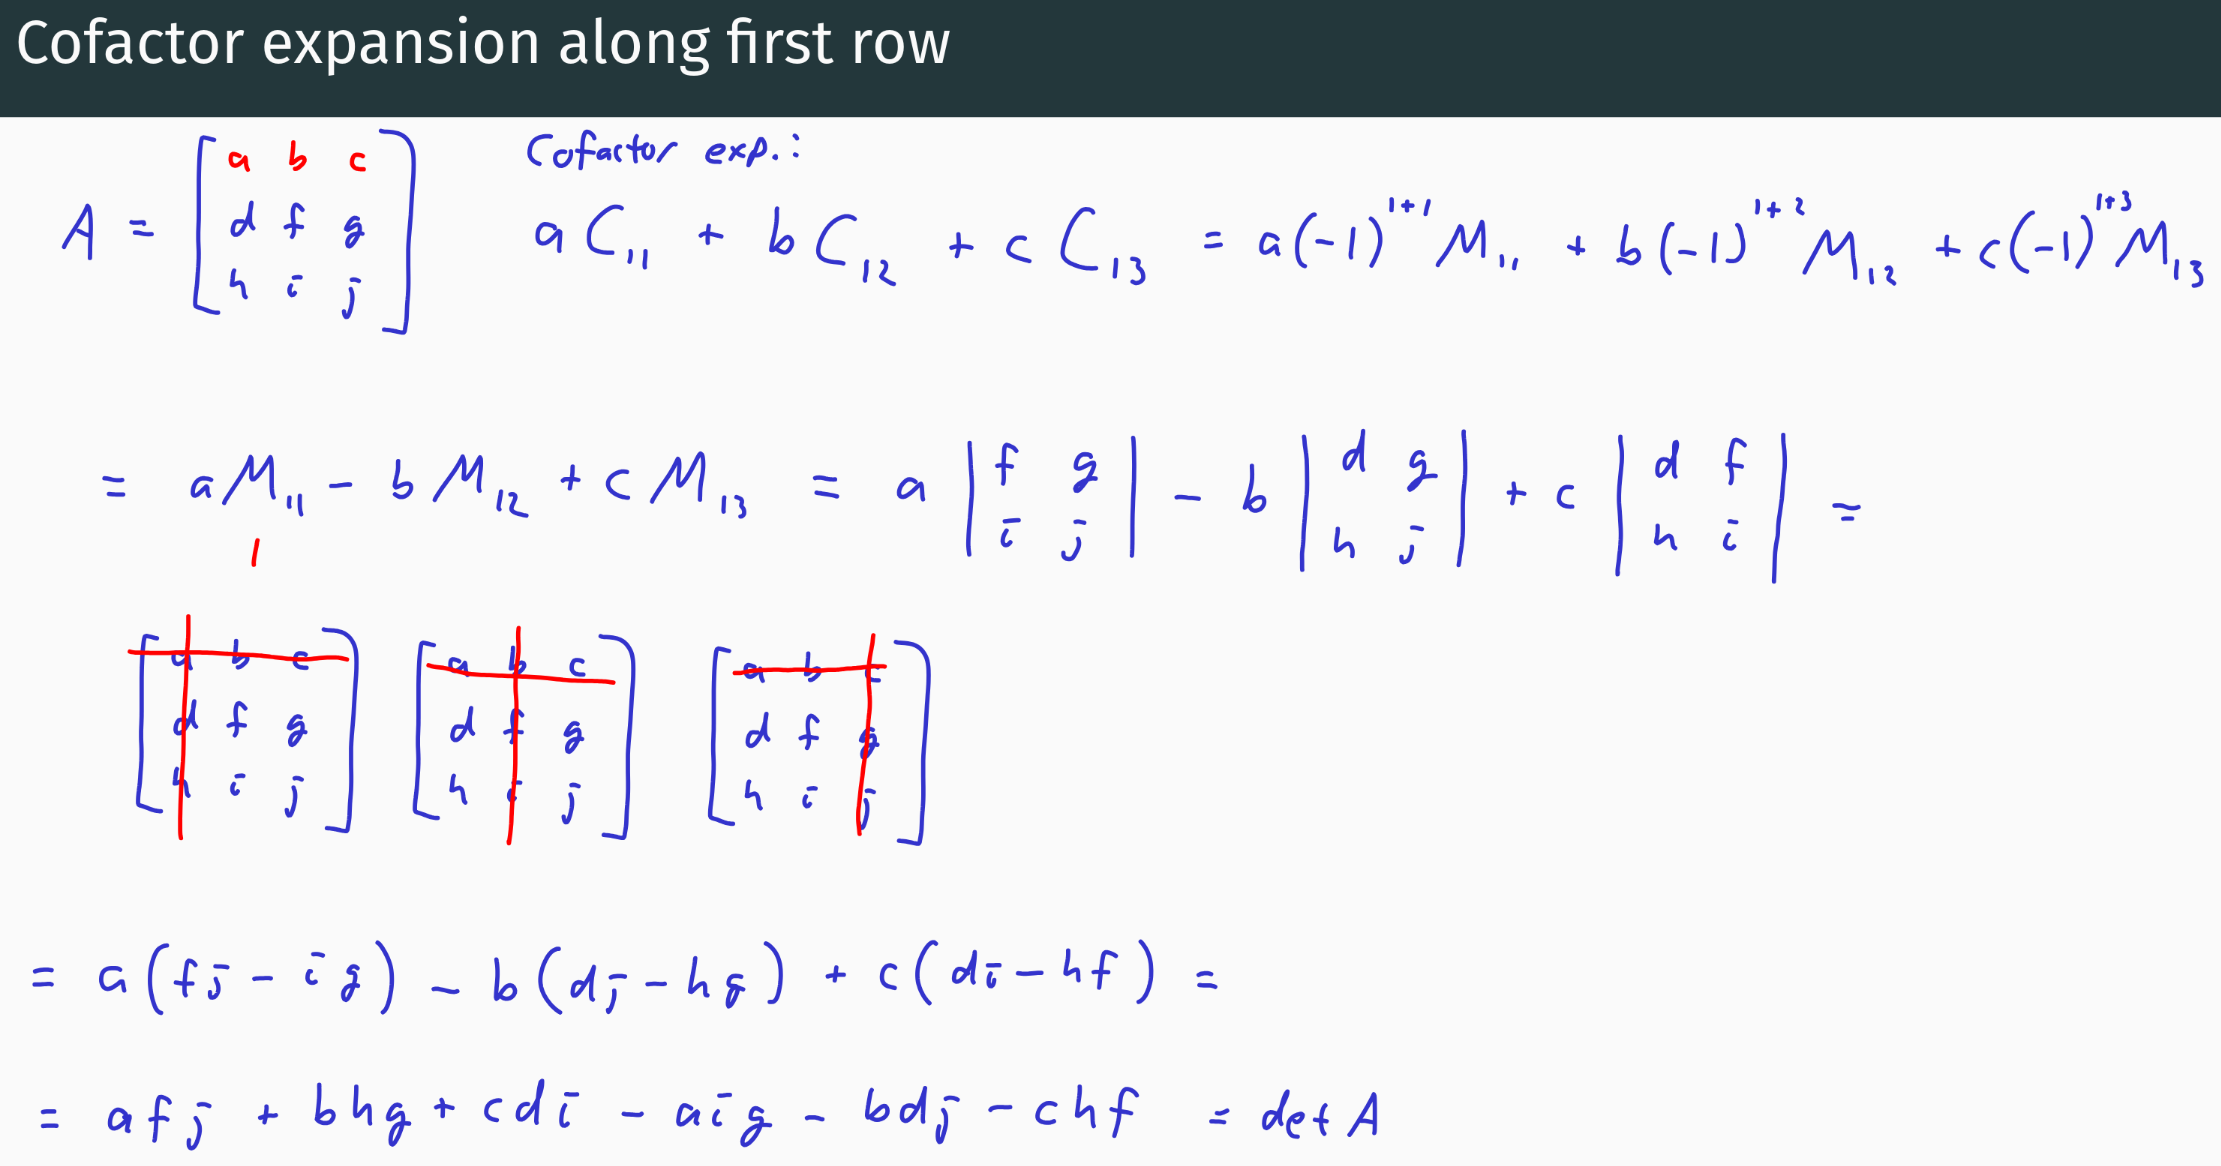
\includegraphics[width=.9\linewidth]{./images/cofactor-expansion-along-the-first-row.png}
\end{center}

\begin{center}
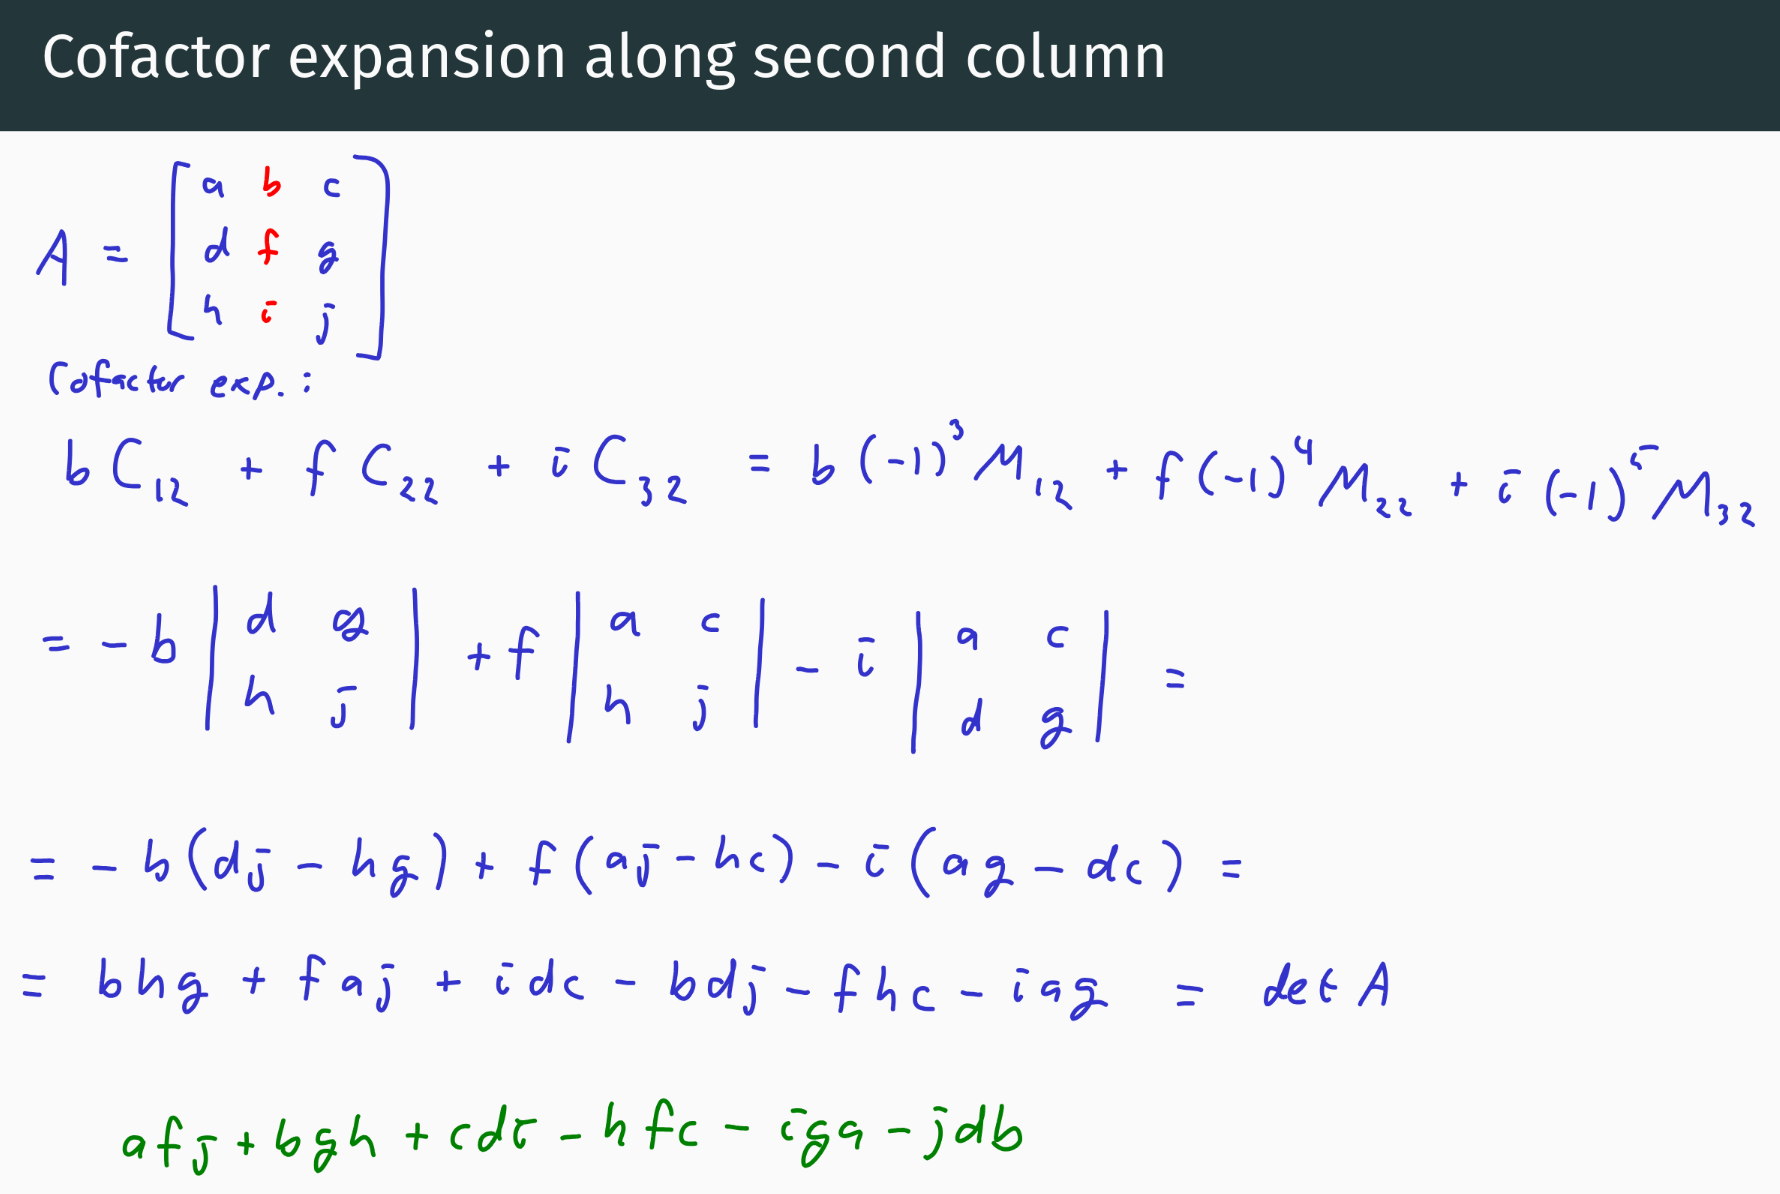
\includegraphics[width=.9\linewidth]{./images/cofactor-expansion-along-the-second-column.png}
\end{center}

\subsubsection{Theorem}
\label{sec:orgfd63a65}
Let \(A\) be an \(n \times n\) matrix. The cofactor expansion along any of its rows or any of its columns will yield the same number.

\subsection{Determinant of a matrix (\(\det A\))}
\label{sec:orgd8327c3}
The \textbf{determinant} \(\det A\) or \(|A|\) of a \textbf{square} matrix \(A\) is a real number.

\subsubsection{Determinant of a \(2 \times 2\) matrix}
\label{sec:org9d0b8b0}
\begin{center}
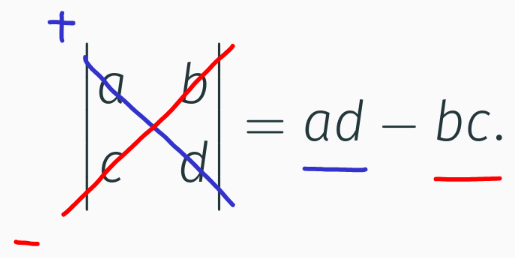
\includegraphics[width=.9\linewidth]{./images/determinant-of-a-2-by-2-matrix.png}
\end{center}

\subsubsection{Determinant of a \(3 \times 3\) matrix}
\label{sec:org1230a70}
\begin{center}
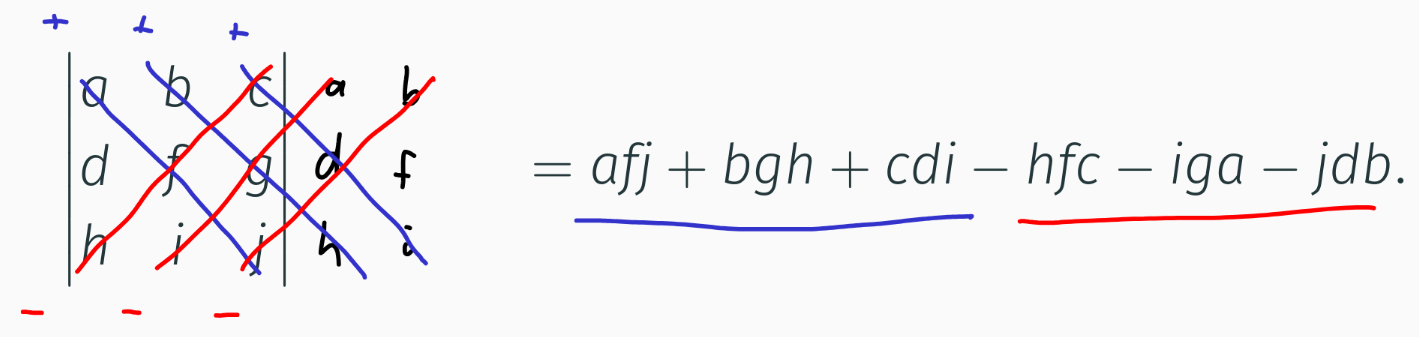
\includegraphics[width=.9\linewidth]{./images/determinant-of-a-3-by-3-matrix.png}
\end{center}

\subsubsection{Definition}
\label{sec:orgc612725}
Let \(A\) be an \(n \times n\) matrix.
\begin{itemize}
\item If \(n = 1\), i.e. \(A = [a]\), we define \(\det A = a\)
\item If \(n \ge 2\), we define \(\det A\) as the number obtained from the cofactor expansion along any row or column of \(A\).
\end{itemize}

\subsubsection{Triangular matrices and diagonal matrices}
\label{sec:org212f30a}
The determinant of a triangular matrix or a diagonal matrix is the product of all the diagonal elements in the matrix.

\subsubsection{Relationship to invertibility}
\label{sec:orgb3ecfbd}
Let \(A\) be an \(n \times n\) matrix. \(A\) is invertible \textbf{if and only if} \(\det A \ne 0\). Hence, \(A\) is singular \textbf{if and only if} \(\det A = 0\).

\subsubsection{Relationship to homogeneous systems}
\label{sec:orgd7124ae}
Let \(A \boldsymbol{x} = \boldsymbol{0}\) be a homogeneous system.

\begin{itemize}
\item \(A \boldsymbol{x} = \boldsymbol{0}\) has a unique solution given by \(\boldsymbol{x} = \boldsymbol{0}\) \textbf{if and only if} \(\det A \ne 0\).
\item \(A \boldsymbol{x} = \boldsymbol{0}\) has infinitely many solutions \textbf{if and only if} \(\det A = 0\).
\end{itemize}

\subsubsection{Rules for the manipulation of determinants}
\label{sec:org3fcafaf}
\[\det (AB) = \det A \cdot \det B\]
\[\det A = \det A^T\]
\[\det A^{-1} = \frac{1}{\det A}\]
\[\det (kA) = k \det A\]

\subsection{Eigenvalues of a matrix (\(\lambda\))}
\label{sec:org2bacd94}
Given an \(n \times n\) matrix \(A\), the eigenvalue is the \(\lambda\) term when finding an \(n \times 1\) vector \(\boldsymbol{x}\) such that \(A \boldsymbol{x} = \lambda \boldsymbol{x}\), where \(\lambda\) is a real or complex number.

\subsection{Eigenvector of a matrix (\(\boldsymbol{x}\))}
\label{sec:org337fca7}
Given an \(n \times n\) matrix \(A\), the eigenvector is the \(n \times 1\) vector \(\boldsymbol{x}\) such that \(A \boldsymbol{x} = \lambda \boldsymbol{x}\), where \(\lambda\) is a real or complex number.

\subsection{Characteristic equation of a matrix}
\label{sec:orgeb879d3}
Given an \(n \times n\) matrix \(A\), the equation below is the characteristic equation of matrix \(A\):
\[\det (A - \lambda I) = 0\]

This equation is used to find the eigenvalues (\(\lambda\)) of \(A\). The characteristic equation is a polynomial equation of order \(n\) and the matrix \(A\) can have up to \(n\) distinct eigenvalues.

\subsection{Diagonalisable matrix}
\label{sec:org460c3ee}
An \(n \times n\) matrix \(A\) is said to be \textbf{diagonalisable} if there exists an invertible matrix \(P\) such that \(D\) is a diagonal matrix:
\[D = P^{-1} A P\]
\[A = PDP^{-1}\]

Where:
\begin{displaymath}
D = \begin{bmatrix}
\lambda_1 & 0 & 0 & 0 & 0 \\
0 & \lambda_2 & 0 & 0 & 0 \\
\vdots & \vdots & \ddots & \vdots & \vdots \\
0 & 0 & 0 & \lambda_{n-1} & 0 \\
0 & 0 & 0 & 0 & \lambda_{n}
\end{bmatrix}
\end{displaymath}

\begin{displaymath}
P = \begin{bmatrix}
\boldsymbol{x}_1 & \boldsymbol{x}_2 & \ldots \boldsymbol{x}_{n-1} & \boldsymbol{x}_{n}
\end{bmatrix}
\end{displaymath}

\(\lambda\) are the eigenvalues of the matrix and \(\boldsymbol{x}\) are the corresponding eigenvectors of the matrix.
\\[0pt]

A matrix is diagonalisable \textbf{if and only if} \(A\) has \(n\) linearly independent eigenvectors.

\subsubsection{For symmetric matrices}
\label{sec:org2ebed4d}
If \(A\) is a symmetric matrix, i.e. \(A = A^T\), then:
\[P^{-1} = P^T\]
\[A = PDP^T\]

\subsection{Vector}
\label{sec:orgacf6c3a}
A vector is a quantity that has magnitude and direction.

\subsubsection{Notation}
\label{sec:orge1ccc18}
Let \(\boldsymbol{u}\) be a vector given by the directed line \(\overrightarrow{PQ}\).
\begin{center}
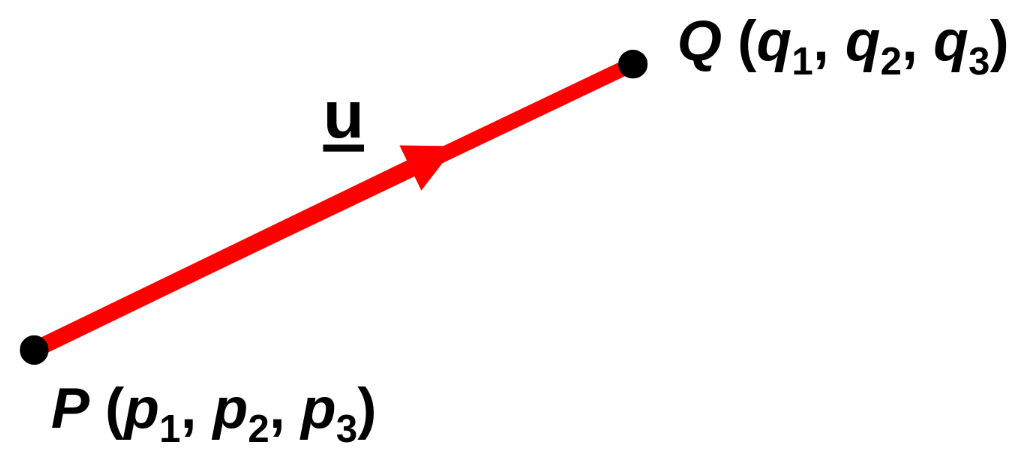
\includegraphics[width=.9\linewidth]{./images/vector-notation-line-pq.png}
\end{center}

\[\boldsymbol{u} = \overrightarrow{PQ} = (q_1 - p_1) \boldsymbol{i} + (q_2 - p_2) \boldsymbol{j} + (q_3 - p_3) \boldsymbol{k}\]

\subsection{Vector addition}
\label{sec:orgd62292b}
If
\[\boldsymbol{u} = a \boldsymbol{i} + b \boldsymbol{j} + c \boldsymbol{k} = (a, b, c)\]
\[\boldsymbol{v} = p \boldsymbol{i} + q \boldsymbol{j} + r \boldsymbol{k} = (p, q, r)\]

Then:
\[\boldsymbol{u} + \boldsymbol{v} = (a + p) \boldsymbol{i} + (b + q) \boldsymbol{j} + (c + r) \boldsymbol{k} = (a + p, b + q, c + r)\]

\begin{center}
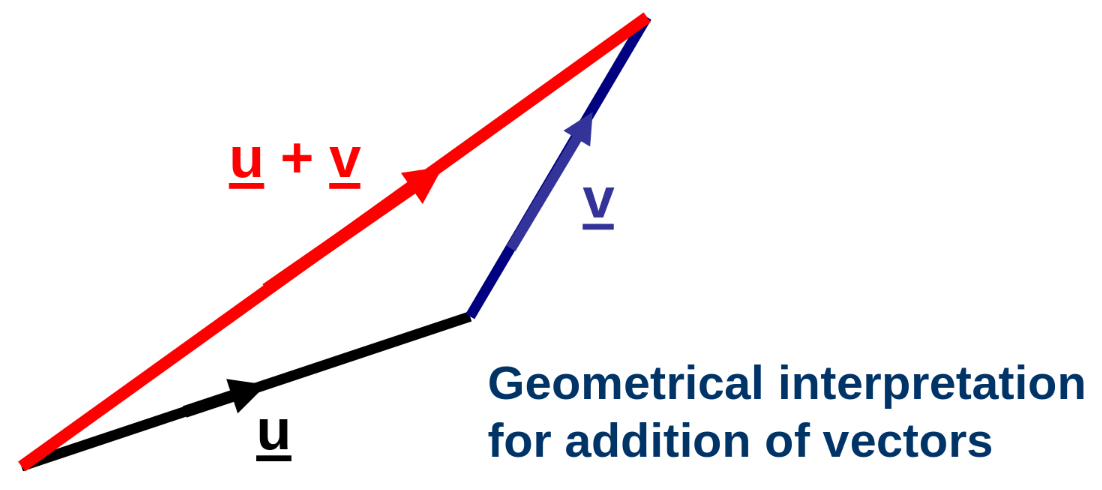
\includegraphics[width=.9\linewidth]{./images/addition-of-vectors-geometrical-interpretation.png}
\end{center}

\subsection{Magnitude of a vector (\(| \boldsymbol{x} |\))}
\label{sec:orgbe70de5}
If \(\boldsymbol{x} = (x_1, x_2, x_3)\), then:
\[| \boldsymbol{x} | = \sqrt{x_1^2 + x_2^2 + x_3^2}\]

\subsection{Norm of a vector (\(|| \boldsymbol{x} ||\))}
\label{sec:org49f28dd}
The norm of a vector gives its magnitude.
\begin{displaymath}
\text{If } \boldsymbol{x} = \begin{bmatrix}
x_1 \\
x_2 \\
\vdots \\
x_n
\end{bmatrix},
\end{displaymath}

Then:
\[|| \boldsymbol{x} || = \sqrt{x_1^2 + x_2^2 + \cdots + x_n^2}\]

\subsection{Multiplication of a vector with a scalar}
\label{sec:org8361a89}
Let \(\boldsymbol{u}\) be a vector \((a, b, c)\) and \(k \in \mathbb{R}\), then:
\[k \boldsymbol{u} = k (a, b, c) = (ka, kb, kc)\]
\[|k \boldsymbol{u}| = |k| |\boldsymbol{u}|\]

If \(k\) is positive, then \(k \boldsymbol{u}\) points in the \textbf{same} direction as \(\boldsymbol{u}\).

If \(k\) is negative, then \(k \boldsymbol{u}\) points in the \textbf{opposite} direction as \(\boldsymbol{u}\).

\subsection{Unit vector}
\label{sec:orgc8cfd56}
Let \(\boldsymbol{u}\) be a vector \((a, b, c)\), then the \textbf{unit} vector \(\boldsymbol{v}\) is given by:
\begin{align*}
\boldsymbol{v} &= \frac{1}{|\boldsymbol{u}|} \boldsymbol{u} \\
&= \frac{1}{\sqrt{a^2 + b^2 + c^2}} (a, b, c) \\
&= \frac{a}{a^2 + b^2 + c^2} \boldsymbol{i} + \frac{b}{a^2 + b^2 + c^2} \boldsymbol{j} + \frac{c}{a^2 + b^2 + c^2} \boldsymbol{k}
\end{align*}

We say that \(\boldsymbol{v}\) is obtained by normalising \(\boldsymbol{u}\).

\subsection{Dot product}
\label{sec:orgd904f8b}
Let \(\boldsymbol{u} = (a, b, c)\) and \(\boldsymbol{v} = (p, q, r)\) be two vectors. We define the dot product \(\boldsymbol{u} \cdot \boldsymbol{v} = ap + bq + cr\).

\[(a, b, c) \cdot (p, q, r) = ap + bq + cr\]
\begin{align*}
\boldsymbol{u} \cdot \boldsymbol{u} &= (a, b, c) \cdot (a, b, c) \\
&= a^2 + b^2 + c^2 \\
&= | \boldsymbol{u} |^2
\end{align*}
\[(\alpha \boldsymbol{u} + \beta \boldsymbol{v}) \cdot (\gamma \boldsymbol{p} + \epsilon \boldsymbol{q}) = \alpha \gamma \boldsymbol{u} \cdot \boldsymbol{p} + \alpha \epsilon \boldsymbol{u} \cdot \boldsymbol{p} + \beta \gamma \boldsymbol{v} \cdot \boldsymbol{p} + \beta \epsilon \boldsymbol{v} \cdot \boldsymbol{p}\]
\[\boldsymbol{u} \cdot \boldsymbol{v} = | \boldsymbol{u} | | \boldsymbol{v} | \cos \theta\]

Where:
\begin{itemize}
\item \(\theta\) is the angle between \(\boldsymbol{u}\) and \(\boldsymbol{v}\)
\end{itemize}

If \(\boldsymbol{u} \cdot \boldsymbol{v}\) is zero then \(\boldsymbol{u}\) and \(\boldsymbol{v}\) are perpendicular.

 \newpage

\subsection{Cross product}
\label{sec:orga3e7d3f}
Let \(\boldsymbol{u} = (a, b, c)\) and \(\boldsymbol{v} = (p, q, r)\) be two vectors. The cross product of a vector is the determinant of the matrix when laying the vectors out as shown below:

\begin{align*}
\boldsymbol{u} \times \boldsymbol{v}
&= (a, b, c) \times (p, q, r) \\
&= \begin{vmatrix}
\boldsymbol{i} & \boldsymbol{j} & \boldsymbol{k} \\
a & b & c \\
p & q & r
\end{vmatrix} \\
&= (br - cq) \boldsymbol{i} + (cp - ar) \boldsymbol{j} + (aq - bp) \boldsymbol{k} \\
&= (br - cq, cp - ar, aq - bp) \\
&= |\boldsymbol{u}| |\boldsymbol{v}| \cos \theta
\end{align*}

Where:
\begin{itemize}
\item \(\theta\) is the angle between \(\boldsymbol{u}\) and \(\boldsymbol{v}\)
\end{itemize}

The resulting vector \(\boldsymbol{u} \times \boldsymbol{v}\) from the cross product is perpendicular to both \(\boldsymbol{u}\) and \(\boldsymbol{v}\).

\begin{center}
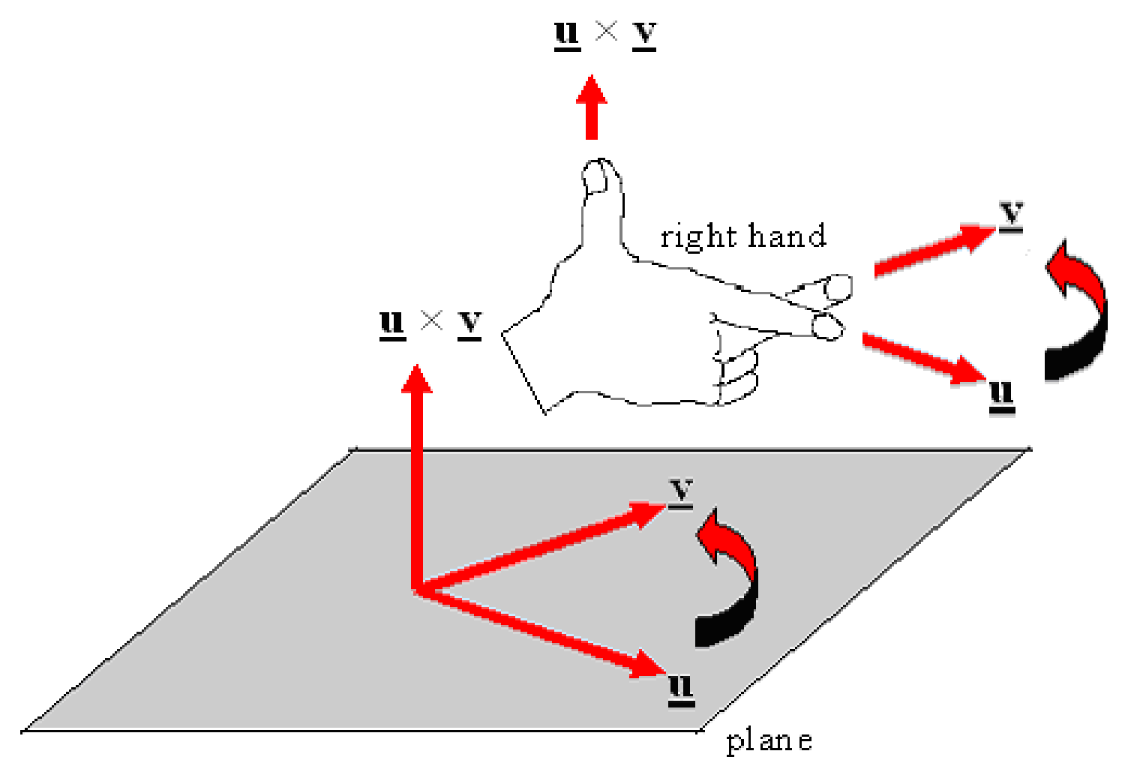
\includegraphics[width=.9\linewidth]{./images/cross-product-right-hand-rule.png}
\end{center}

\subsection{Plane}
\label{sec:org9c6a1db}
The equation of a plane is given in the forms below:
\[ax + by + cz = k, k \in \mathbb{R}\]
\[\vec{n} \cdot \vec{r} = 0\]

Where:
\begin{itemize}
\item \(\vec{n}\) is the normal vector of the plane, given by \((a, b, c)\)
\item \(\vec{r}\) is the position vector of any point on the plane
\end{itemize}

\subsubsection{Parametrising the plane}
\label{sec:org8f2b4cc}
\[x = \alpha_1 s + \beta_1 u + \gamma_1\]
\[y = \alpha_2 s + \beta_2 u + \gamma_2\]
\[z = \alpha_3 s + \beta_3 u + \gamma_3\]

Where:
\begin{itemize}
\item \(s\) and \(u\) are free parameters, i.e. \(s, u \in \mathbb{R}\).
\item \(x, y\) and \(z\) are expressed in terms of linear functions of \(s\) and \(u\).
\end{itemize}

\subsection{Surfaces}
\label{sec:org331bce5}
Points \((x, y, z)\) on a surface in 3D space may be described by a single equation in \(x, y\) and \(z\), which is:
\[F(x, y, z) = k, k \in \mathbb{R}\]

In parametric form, the \(x, y\) and \(z\) coordinates on a surface are described by functions of two parameters \(s\) and \(u\), namely:
\[x = f(s, u)\]
\[y = g(s, u)\]
\[z = h(s, u)\]

The functions above are the solutions of \(F(x, y, z) = k\). For a plane, \(f, g\) and \(h\) are linear functions of \(s\) and \(u\).

\subsubsection{Examples}
\label{sec:orgdfb3a54}
Plane (flat) surface:
\[2x + y + z = 1\]

Spherical surface:
\[(x - 1)^2 + (y - 2)^2 (z - 3)^2 = 16\]

\subsubsection{Parametrising the surface}
\label{sec:orgf36d433}
Let the surface \(S\) be given by \((x - 1)^2 + (y - 2)^2 + (z - 3)^2 = 16\). Let \(z - 3 = \rho\).

\[(x - 1)^2 + (y - 2)^2 + (z - 3)^2 = 16\]
\[(x - 1)^2 + (y - 2)^2 + \rho^2 = 16\]
\[(x - 1)^2 + (y - 2)^2 = 16 - \rho^2 \tag{1}\]

The left-hand side of the equation is always positive, hence:
\[16 - \rho^2 \ge 0\]
\[-4 \le \rho \le 4\]

Using the trigonometric identity:
\[\cos^2 \theta + \sin^2 = 1\]

Let \(a = \sqrt{16 - \rho^2}\):
\[(a \cos \theta)^2 + (a \sin \theta)^2 = a^2 \tag{2}\]

Comparing \((1)\) and \((2)\):
\[x - 1 = \sqrt{16 - \rho^2} \cos \theta\]
\[y - 2 = \sqrt{16 - \rho^2} \sin \theta\]

Hence, a possible parametric representation is:
\begin{displaymath}
\left. \begin{array}{l}
x = 1 + \sqrt{16 - \rho^2} \cos \theta \\
y = 2 + \sqrt{16 - \rho^2} \sin \theta \\
z = 3 + \rho
\end{array} \right\} \text{ for } \begin{array}{c}
-4 \le \rho \le 4 \\
0 \le \theta < 2 \pi
\end{array}
\end{displaymath}

\subsection{Curves in 3D}
\label{sec:orgac6b9f6}
A curve may be formed by the intersection of two surfaces.
As a surface is described by an equation in \(x, y\) and \(z\), finding all the points on a curve is like solving 2 equations in 3 unknowns \(x, y\) and \(z\).
One of the unknowns can be set to be a free parameter to solve for the other two unknowns (in terms of the free parameter).

Hence, all points on a curve can be expressed in parametric form as:
\[x = F(s)\]
\[y = G(s)\]
\[z = H(s)\]

For a straight line:
\[x = at + p\]
\[y = bt + q\]
\[z = ct + r\]

Where:
\begin{itemize}
\item \(s\) and \(t\) are free parameters, i.e. \(s, t \in \mathbb{R}\)
\end{itemize}

\subsection{Derivative of a vector function}
\label{sec:orgc90ba8c}
Let \(f\) be a scalar function \(f(x)\) and \(\boldsymbol{F}\) be a vector function \(\boldsymbol{F}(u)\). The derivative of a scalar function is:
\[f'(x) = \frac{df}{dx} = \lim_{h \rightarrow 0} \frac{f(x + h) - f(x)}{h}\]

Where:
\begin{itemize}
\item \(f(x + h) - f(x)\) is the change in output
\item \(h\) is the change in input
\end{itemize}

Likewise, the derivative of the vector function follows as:
\[\boldsymbol{F}'(u) = \frac{d \boldsymbol{F}}{du} = \lim_{h \rightarrow 0} \frac{\boldsymbol{F}(u + h) - \boldsymbol{F}(u)}{h}\]

For \(\boldsymbol{F}(u) = (p(u), q(u), r(u))\):
\[\frac{d \boldsymbol{F}}{du} = \left(\frac{dp}{du}, \frac{dq}{du}, \frac{dr}{du} \right)\]

\subsubsection{Example}
\label{sec:org3958f92}
\[\boldsymbol{F}(u) = (\sin 2u, u^3 + 2u^2, 2u)\]
\[\frac{d \boldsymbol{F}}{du} = (2 \cos 2u, 3u^2 + 4u, 2)\]
\[\frac{d^2 \boldsymbol{F}}{du^2} = (-4 \sin 2u, 6u + 4, 0)\]

\subsubsection{Product rule}
\label{sec:org9c67a8a}
Let \(g\) be a scalar function of one variable \(x\) and \(\boldsymbol{G}\) is a vector function of \(x\).
\[\frac{d}{dx} g(x) \boldsymbol{G}(x) = g(x) \frac{d \boldsymbol{G}}{dx} + \frac{dg}{dx} \boldsymbol{G}\]

\subsubsection{Chain rule}
\label{sec:org191578a}
Let \(F\) be a vector function given by \(F(u) = f(x(u), y(u), z(u))\):
\[\frac{dF}{du} = \frac{\partial f}{\partial x} \cdot \frac{dx}{du} + \frac{\partial f}{\partial y} \cdot \frac{dy}{du} + \frac{\partial f}{\partial z} \cdot \frac{dz}{du}\]

\subsection{Motion of a particle}
\label{sec:orgcf77f8e}
\begin{center}
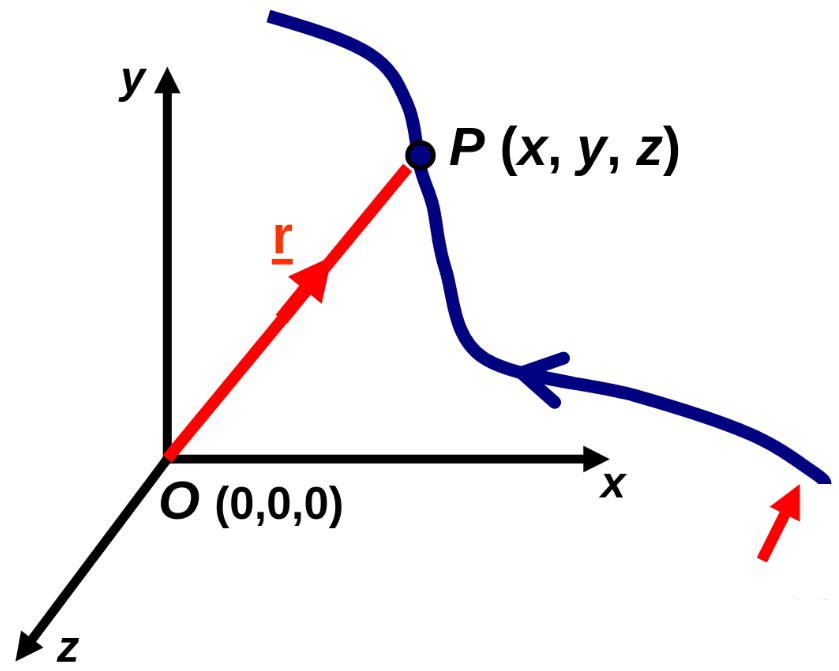
\includegraphics[width=.9\linewidth]{./images/motion-of-a-particle.png}
\end{center}

\subsubsection{Position of the particle}
\label{sec:org1ae82b9}
The position of a particle is changing with respect to time (\(t\)):
\begin{align*}
x &= xt \\
y &= yt \\
z &= zt
\end{align*}

\subsubsection{Position or displacement of the particle}
\label{sec:org970f418}
The position or displacement of the particle is with respect to the origin (\(O\)):
\begin{align*}
\boldsymbol{r} (t) &= (x(t) - 0) \boldsymbol{i} + (y(t) - 0) \boldsymbol{j} - (z(t) - 0) \boldsymbol{k} \\
&= (x(t), y(t), z(t)) \\
&= x(t) \boldsymbol{i} + y(t) + \boldsymbol{j} + z(t) \boldsymbol{k}
\end{align*}

\subsubsection{Velocity of the particle}
\label{sec:orgfbc8e7b}
Velocity is the rate of change of displacement with respect to time (\(t\)):
\[\frac{d \boldsymbol{r}}{dt} = \frac{dx}{dt} \boldsymbol{i} + \frac{dy}{dt} \boldsymbol{j} + \frac{dz}{dt} \boldsymbol{k}\]

\subsubsection{Speed of the particle}
\label{sec:orgae5fde3}
Speed is the magnitude of the velocity:
\[\left| \frac{d \boldsymbol{r}}{dt} \right| = \sqrt{\left(\frac{dx}{dt} \right)^2 + \left(\frac{dy}{dt} \right)^2 + \left(\frac{dz}{dt} \right)^2}\]

\subsubsection{Acceleration of the particle}
\label{sec:orgd183267}
Acceleration is the rate of change of velocity with respect to time.
\[\frac{d^2 \boldsymbol{r}}{dt^2} = \frac{d^2 x}{dt^2} \boldsymbol{i} + \frac{d^2 y}{dt^2} \boldsymbol{j} + \frac{d^2 z}{dt^2} \boldsymbol{k}\]

 \newpage

\subsection{Newton's second law}
\label{sec:org3c22052}
Let \(\boldsymbol{F} = (F_x, F_y, F_z)\):
\begin{align*}
\boldsymbol{F} &= m \frac{d^2 \boldsymbol{r}}{dt^2} \\
&= m \left(\frac{d^2 x}{dt^2}, \frac{d^2 y}{dt^2}, \frac{d^2 z}{dt} \right) \\
&= ma
\end{align*}
\begin{align*}
F_x &= m \frac{d^2 x}{dt^2} \\
F_y &= m \frac{d^2 y}{dt^2} \\
F_z &= \frac{d^2 z}{dt}
\end{align*}

Where:
\begin{itemize}
\item \(\boldsymbol{F}\) is the force vector on the object
\item \(m\) is the mass of the object
\item \(\boldsymbol{r}\) is the displacement vector of the object
\item \(t\) is the time
\item \(a\) is the acceleration of the object
\end{itemize}

\subsection{Vector differential operator (\(\nabla\))}
\label{sec:orge2d94fe}
The vector differential operator is defined as:
\begin{align*}
\nabla &= \frac{\partial}{\partial x} \boldsymbol{i} + \frac{\partial}{\partial y} \boldsymbol{j} + \frac{\partial}{\partial z} \boldsymbol{k} \\
&= \left(\frac{\partial}{\partial x}, \frac{\partial}{\partial y}, \frac{\partial}{\partial z} \right)
\end{align*}

\subsection{Gradient operator (grad)}
\label{sec:orga2b3c9e}
The gradient operator is essentially the same as the \(\nabla\) operator.
\[\text{grad } f = \nabla f = \left(\frac{\partial f}{\partial x}, \frac{\partial f}{\partial y}, \frac{\partial f}{\partial z} \right)\]

\subsection{Normal vectors}
\label{sec:org82fece5}

\subsubsection{Curves}
\label{sec:org6f1ed1b}
A curve in 2D space is given in the form \(F(x, y) = c, c \in \mathbb{R}\). \textbf{A} normal vector to the curve is given by:
\[\nabla F = \left(\frac{\partial F}{\partial x}, \frac{\partial F}{\partial y} \right)\]

\subsubsection{Surfaces}
\label{sec:orgf2a49fa}
A surface in 3D space is given in the form \(F(x, y, z) = c, c \in \mathbb{R}\). \textbf{A} normal vector to the curve is given by:
\[\left. \nabla F \right|_{(x, y, z) = (x_0, y_0, z_0)}\]

\subsection{Divergence operator (div)}
\label{sec:orgdc1ace2}
Let \(\boldsymbol{F}\) be a vector function:
\begin{align*}
\text{div } \boldsymbol{F} &= \nabla \cdot \boldsymbol{F} \\
&= \left(\frac{\partial}{\partial x}, \frac{\partial}{\partial y}, \frac{\partial}{\partial z} \right) \cdot \boldsymbol{F}
\end{align*}

\subsection{Curl operator (curl)}
\label{sec:org2ce398f}
Let \(\boldsymbol{F}\) be a vector function:
\begin{align*}
\text{curl } \boldsymbol{F} &= \nabla \times \boldsymbol{F} \\
&= \left(\frac{\partial}{\partial x}, \frac{\partial}{\partial y}, \frac{\partial}{\partial z} \right) \times \boldsymbol{F}
\end{align*}

\subsection{Laplacian operator (\(\nabla^2\))}
\label{sec:org44ee998}
\begin{align*}
\nabla^2 = \nabla \cdot \nabla = \left(\frac{\partial^2}{\partial x^2}, \frac{\partial^2}{\partial y^2}, \frac{\partial^2}{\partial z^2}\right)
\end{align*}

\subsection{Leibniz theorem}
\label{sec:org7d2e3d5}
\label{orgc41eb53}
If we can find a function \(F(x)\) such that \(\frac{dF}{dx} = f(x)\), then:
\[\int_a^b f (x) \, dx = F(b) - F(a)\]

\subsection{Line element (\(ds\))}
\label{sec:orge8d32d1}
For a line \(\boldsymbol{r}\) that can be parametrised with \(t\):
\[ds = \left| \left| \frac{d \boldsymbol{r}}{dt} \right| \right|\]

For example:
\begin{align*}
\boldsymbol{r} &= (x, y, z) \\
ds &= \left| \left| \frac{d}{dt} (x, y, z) \right| \right| \\
&= \left| \left| \left(\frac{dx}{dt}, \frac{dy}{dt}, \frac{dz}{dt} \right) \right| \right| \\
&= \sqrt{\left(\frac{dx}{dt} \right)^2 + \left(\frac{dy}{dt} \right)^2 + \left(\frac{dz}{dt} \right)^2}
\end{align*}

\subsection{Length of a curve (arc length)}
\label{sec:orgf36fa35}
For a smooth curve \(C\):
\[\int_C \, ds\]

Where:
\begin{itemize}
\item \(\int_C \, ds\) in context of a particle's motion is the distance travelled by the particle.
\end{itemize}

\subsection{Line integral of a scalar function (area under a curve)}
\label{sec:org94700ab}
\begin{center}
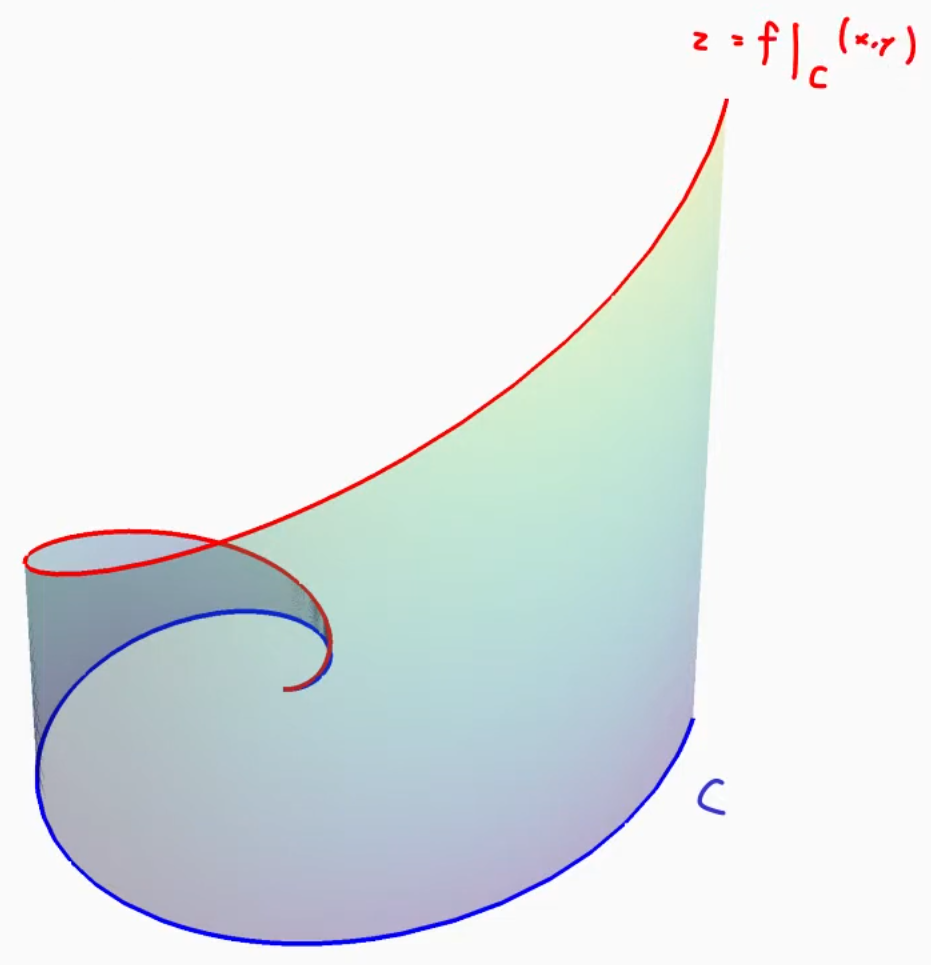
\includegraphics[width=.9\linewidth]{./images/line-integral-of-a-scalar-function.png}
\end{center}
For a smooth curve \(C\) and a scalar function \(f\):
\[\int_C f(\boldsymbol{x}) \, ds = \int_C f(x, y, z) \, ds\]

 \newpage

\subsection{Line integral of a vector function (work done)}
\label{sec:orgffa09c4}
The line integral of a vector function can be thought of as the work done by the vector function.
For a smooth curve \(C\) parametrised by \(\boldsymbol{x} = \boldsymbol{r} (t), t \in [a, b]\) and a vector function \(\boldsymbol{F}\):
\begin{align*}
\int_C \boldsymbol{F} \cdot d \boldsymbol{r} &= \int_C \boldsymbol{F} \cdot \boldsymbol{U} \, ds \\
&= \int_a^b \boldsymbol{F} (\boldsymbol{r} (t)) \cdot \boldsymbol{r'} (t) \, dt
\end{align*}

Where:
\begin{itemize}
\item \(d \boldsymbol{r}\) is the infinitesimal position or displacement vector in the context of a particle's motion.
\item \(\boldsymbol{U}\) is the unit vector representing the direction of travel in the context of a particle's motion.
\item \(ds\) is the infinitesimal distance of each section of the curve, or the infinitesimal arc length of the curve.
\item \(\boldsymbol{r}\) is the position vector of the particle in the context of a particle's motion.
\item \(\boldsymbol{r'}\) is the derivative of the position vector of the particle with respect to time \(t\) in the context of a particle's motion. In other words, \(\boldsymbol{r'}\) is the velocity of the particle.
\end{itemize}

\subsection{Infinitesimal surface area element (\(dS\))}
\label{sec:org8742a32}
If the equation for a surface \(S\) can be written as \(z = f(x, y)\), then the relationship between the infinitesimal \textbf{surface area} element \(dS\) and the infinitesimal \textbf{area} element \(dA\) is:
\[dS = \sqrt{1 + \left(\frac{\partial f}{\partial x} \right)^2 + \left(\frac{\partial f}{\partial y} \right)^2} \, dA\]

\subsection{Surface area of a surface}
\label{sec:orgaf80b46}
For a smooth surface \(S\):
\[\iint_S \, dS\]

Where:
\begin{itemize}
\item \(dS\) is the infinitesimal surface area element.
\end{itemize}

\subsection{Surface integral of a scalar function}
\label{sec:org587aedd}
For a smooth surface \(S\) and a scalar function \(f(\boldsymbol{x})\), where \(\boldsymbol{x} = (x, y) = (r \cos \theta, r \sin \theta)\):
\begin{align*}
\iint_S f(\boldsymbol{x}) \, dS &= \iint_R f(x, y) dy dx \\
&= \iint_R f(r, \theta) \, r dr d \theta
\end{align*}

Where:
\begin{itemize}
\item \(dS\) is the infinitesimal surface area element.
\end{itemize}

\subsection{Surface integral of a vector function (flux)}
\label{sec:org1638eef}
The surface integral of a vector function can be thought of as the flux through the surface.
For a smooth surface \(S\) and a vector function \(\boldsymbol{F}\):
\[\iint_S \boldsymbol{F} \cdot \hat{n} \, dS\]

Where:
\begin{itemize}
\item \(\hat{n}\) is the unit normal vector to the surface, i.e. the vector is perpendicular to the surface, and has a magnitude of 1.
\item \(dS\) is the infinitesimal surface area element.
\end{itemize}

\subsection{Volume integral}
\label{sec:orgbe1152b}
For a volume \(T\):
\[\iiint_T dV\]

Where:
\begin{itemize}
\item \(dV\) is the infinitesimal volume element.
\end{itemize}

 \newpage

\subsection{Green's theorem}
\label{sec:org03a9068}
\[\oint_C f(x, y) \, dx + g (x, y) \, dy = \iint_R \left(\frac{\partial g}{\partial x} - \frac{\partial f}{\partial y} \right) \, dx dy\]

Where:
\begin{itemize}
\item \(C\) is a closed curve that is positively oriented. A positively oriented curve is a curve that has the region \(R\) bounded by the curve on the \textbf{left} side as we walk along the curve, with our head facing the direction of the curve.
\item \(R\) is the region bounded by the closed curve \(C\).
\end{itemize}

\subsection{Stoke's theorem}
\label{sec:org6da9ce2}
Stoke's theorem essentially states that the line integral of a vector function, or the work done by the vector function, is equal to surface integral of the curl of the vector function. It is the multidimensional version of Green's theorem.
For a smooth curve \(C\) and a vector function \(\boldsymbol{F}\):
\[\oint_C \boldsymbol{F} \cdot d \boldsymbol{r} = \iint_S (\text{curl } \boldsymbol{F}) \cdot \hat{n} \, dS = \iint_S (\nabla \times \boldsymbol{F}) \cdot \hat{n} \, dS\]

Where:
\begin{itemize}
\item \(\hat{n}\) is the unit normal vector to the surface, i.e. a vector that is perpendicular to the surface with a magnitude of 1.
\item \(dS\) is the infinitesimal surface area element.
\end{itemize}

\subsection{Gauss' divergence theorem}
\label{sec:org222b555}
Gauss' divergence theorem essentially states that the surface integral of a vector function, or the flux through a surface, is equal to the volume integral of the divergence of the vector function.
For a smooth surface \(S\) and a vector function \(\boldsymbol{F}\):
\[\iint_S F \cdot \hat{n} \, dS = \iiint_T \text{div } \boldsymbol{F} \, dV = \iiint_T \nabla \cdot \boldsymbol{F} \, dV\]

Where:
\begin{itemize}
\item \(\hat{n}\) is the unit normal vector to the surface, i.e. a vector that is perpendicular to the surface with a magnitude of 1.
\item \(dS\) is the infinitesimal surface area element.
\item \(dV\) is the infinitesimal volume element.
\end{itemize}

\subsection{Conservative vector fields}
\label{sec:org765cc2c}

\subsubsection{Two-dimensional vector fields}
\label{sec:orgdf899b0}
A vector field \(\boldsymbol{F} (x, y) = f(x, y) \boldsymbol{i} + g(x, y) \boldsymbol{j}\) is considered \textbf{conservative} if:
\[\frac{\partial g}{\partial x} = \frac{\partial f}{\partial y}\]

\subsubsection{Vector fields with 3 or more dimensions}
\label{sec:orgc4d1606}
A vector field \(\boldsymbol{F}\) is considered \textbf{conservative} if:
\[\text{curl } \boldsymbol{F} = \nabla \times F = \boldsymbol{0}\]

\subsection{Potential function}
\label{sec:orgffdbb0a}
\begin{itemize}
\item If the vector field \(\boldsymbol{F} (x, y) = f(x, y) \boldsymbol{i} + g(x, y) \boldsymbol{j}\) is conservative, we can find a function \(\phi (x, y)\) such that \(\frac{\partial \phi}{\partial x} = f(x, y)\) and \(\frac{\partial \phi}{\partial y} = g(x, y)\).
\item This function \(\phi (x, y)\) is called the \textbf{potential function} of \(\boldsymbol{F} (x, y)\).
\item With this potential function, we can easily get the integral of the vector field using the \hyperref[orgc41eb53]{Leibniz theorem}.
\end{itemize}

\subsection{Periodic functions}
\label{sec:orge15955f}
Let \(f(x)\) be a well-defined function for \(- \infty < x < \infty\). \(f(x)\) is said to be periodic with period \(p\), where \(p\) is a non-zero constant, if \(f(x)\) satisfies the property:
\[f(x + p) = f(x), x \in \mathbb{R}\]

\subsubsection{Sum and product of periodic functions}
\label{sec:orgc6d4087}
Let \(f(x)\) and \(g(x)\) be periodic with period \(p\). Then:
\begin{itemize}
\item \(f(x) + g(x)\) is periodic with period \(p\)
\item \(f(x) g(x)\) is also periodic with period \(p\)
\end{itemize}

\subsubsection{Integral of a periodic function}
\label{sec:org03714b2}
If \(f(x)\) is periodic with period \(p\), then:
\[\int_{x = c}^{x = c + p} f(x) \, dx \text{ has the same value no matter what } c \text{ is.}\]

\subsubsection{Examples}
\label{sec:org433db83}
\[f(x) = \sin (x), - \infty < x < \infty\]
\[g(x) = \cos (x), - \infty < x < \infty\]

Both of the functions above are periodic with periods of \(2 \pi\), because:
\[\sin(x + 2 \pi) = \sin (x), \quad \cos (x + 2 \pi) = \cos (x)\]

\subsection{Fourier series of a periodic function}
\label{sec:orgb830aea}
The Fourier series of a periodic function \(f(x)\) with period \(2L, L \in \mathbb{R}^+\), is given by the series:
\[a_0 + \sum_{n = 1}^{\infty} \left\{a_n \cos \left( \frac{n \pi x}{L} \right) + b_n \sin \left( \frac{n \pi x}{L} \right) \right\}\]

Where:
\[a_0 = \frac{1}{2L} \int_{\alpha}^{\alpha + 2L} f(x) \, dx\]
\[a_n = \frac{1}{L} \int_{\alpha}^{\alpha + 2L} f(x) \cos \left( \frac{n \pi x}{L} \right) \, dx\]
\[b_n = \frac{1}{L} \int_{\alpha}^{\alpha + 2L} f(x) \sin \left( \frac{n \pi x}{L} \right) \, dx\]
\[n = 1, 2, 3, \ldots\]

\subsection{Condition for a periodic function to be equal to its Fourier series}
\label{sec:org297ae12}
Let a periodic function be \(f(x)\). For \(f(x)\) to be equal to its Fourier series:
\[a_0 + \sum_{n = 1}^{\infty} \left\{a_n \cos \left( \frac{n \pi s}{L} \right) + b_n \sin \left( \frac{n \pi s}{L} \right) \right\} = \frac{1}{2} \left( \lim_{x \rightarrow s^{-}} f(x) + \lim_{x \rightarrow s^{+}} f(x) \right)\]

If \(f(x)\) is continuous at \(x = s\), then the Fourier series of \(f(x)\) at \(x = s\) is equal to \(f(x)\), i.e.
\[a_0 + \sum_{n = 1}^{\infty} \left\{a_n \cos \left( \frac{n \pi x}{L} \right) + b_n \sin \left( \frac{n \pi x}{L} \right) \right\} = f(x) \text{ where } f(x) \text{ is continuous}\]

\subsection{Odd functions}
\label{sec:org04c6972}
A function \(f(x)\) is said to be \textbf{odd} over the interval \(- a < x < a, a \in \mathbb{R}^{+}\) if \(f(-x) = - f(x)\) for \(-a < x < a\).  \\

If \(f(x)\) is \textbf{odd} over \(-a < x < a\), then:
\[\int_{-a}^{a} f(x) \, dx = 0\]

\subsubsection{Example}
\label{sec:org1ceee30}
\[S(x) = \sin \left( \frac{n \pi x}{L} \right) \text{ is odd over } -L < x < L\]

\subsection{Even functions}
\label{sec:orgda8d5a0}
A function \(f(x)\) is said to be \textbf{even} over the interval \(- a < x < a, a \in \mathbb{R}^{+}\) if \(f(-x) = f(x)\) for \(-a < x < a\).  \\

If \(f(x)\) is \textbf{even} over \(-a < x < a\), then:
\[\int_{-a}^{a} f(x) \, dx = 2 \int_0^{2a} f(x) \, dx\]

\subsubsection{Example}
\label{sec:orgc725f77}
\[C(x) = \cos \left( \frac{n \pi x}{L} \right) \text{ is even over } -L < x < L\]

 \newpage

\subsection{Sum and product of even and odd functions}
\label{sec:orgf8c70d5}

\subsubsection{\(f(x)\) and \(g(x)\) are both odd over \(- a < x < a\)}
\label{sec:orgdf23d06}
\begin{itemize}
\item \(f(x) + g(x)\) is also \textbf{odd} over \(- a < x < a\)
\item \(f(x) g(x)\) is \textbf{even} over \(- a < x < a\)
\end{itemize}

\subsubsection{\(f(x)\) and \(g(x)\) are both even over \(- a < x < a\)}
\label{sec:org3f9c0fe}
\begin{itemize}
\item \(f(x) + g(x)\) is also \textbf{even} over \(- a < x < a\)
\item \(f(x) g(x)\) is also \textbf{even} over \(- a < x < a\)
\end{itemize}

\subsubsection{\(f(x)\) is odd while \(g(x)\) is even over \(- a < x < a\)}
\label{sec:orgce172d1}
\begin{itemize}
\item \(f(x) + g(x)\) is neither odd nor even over \(- a < x < a\)
\item \(f(x) g(x)\) is \textbf{odd} over \(- a < x < a\)
\end{itemize}

 \newpage

\subsection{Fourier series of an odd periodic function}
\label{sec:orgf735b9b}
The Fourier series of an \textbf{odd} periodic function \(f(x)\) is called the Fourier sine series, and is given by:
\[\sum_{n = 1}^{\infty} b_n \sin \left( \frac{n \pi x}{L} \right)\]

Where:
\begin{align*}
b_n &= \frac{1}{L} \int_{-L}^{L} f(x) \sin \left( \frac{n \pi x}{L} \right) \, dx \\
&= \frac{2}{L} \int_0^L f(x) \sin \left( \frac{n \pi x}{L} \right) \, dx \quad \because f(x) \text{ and } \sin \left( \frac{n \pi x}{L} \right) \text{ are both odd}
\end{align*}

\subsubsection{Extending a continuous function}
\label{sec:org5175f9c}
Suppose \(g(x)\) is a continuous function over \(0 < x < l, l \in \mathbb{R}\). We can extend \(g(x)\) to become an \textbf{odd} periodic function of period \(2l\) by letting \(g(x) = - g(-x)\):

\[g(x) = \sum_{n = 1}^{\infty} b_n \sin \left( \frac{n \pi x}{l} \right), \quad 0 < x < l\]

Where:
\[b_n = \frac{2}{l} \int_0^l g(x) \sin \left( \frac{n \pi x}{l} \right) \, dx\]
\[n = 1, 2, 3, \ldots\]

 \newpage

\subsection{Fourier series of an even periodic function}
\label{sec:org483497e}
The Fourier series of an \textbf{even} periodic function \(f(x)\) is called the Fourier cosine series, and is given by:
\[a_0 + \sum_{n = 1}^{\infty} a_n \cos \left( \frac{n \pi x}{L} \right)\]

Where:
\begin{align*}
a_0 &= \frac{1}{2L} \int_{-L}^{L} f(x) \, dx \\
&= \frac{1}{L} \int_0^L f(x) \, dx \quad \because f(x) \text{ is even} \\
a_n &= \frac{1}{L} \int_{-L}^{L} f(x) \cos \left( \frac{n \pi x}{L} \right) \, dx \\
&= \frac{2}{L} \int_0^L f(x) \cos \left( \frac{n \pi x}{L} \right) \, dx \quad \because f(x) \text{ and } \cos \left( \frac{n \pi x}{L} \right) \text{ are both even}
\end{align*}

\subsubsection{Extending a continuous function}
\label{sec:org091fc8b}
Suppose \(g(x)\) is a continuous function over \(0 < x < l, l \in \mathbb{R}\). We can extend \(g(x)\) to become an \textbf{even} periodic function of period \(2l\) by letting \(g(x) = g(-x)\):

\[g(x) = a_0 + \sum_{n = 1}^{\infty} a_n \cos \left( \frac{n \pi x}{l} \right), \quad 0 < x < l\]

Where:
\[a_0 = \frac{1}{l} \int_0^l g(x) \, dx\]
\[a_n = \frac{2}{l} \int_0^l g(x) \cos \left( \frac{n \pi x}{l} \right) \, dx\]
\[n = 1, 2, 3, \ldots\]

 \newpage

\subsection{Periodic extensions of continuous functions}
\label{sec:orgff1db93}
\begin{center}
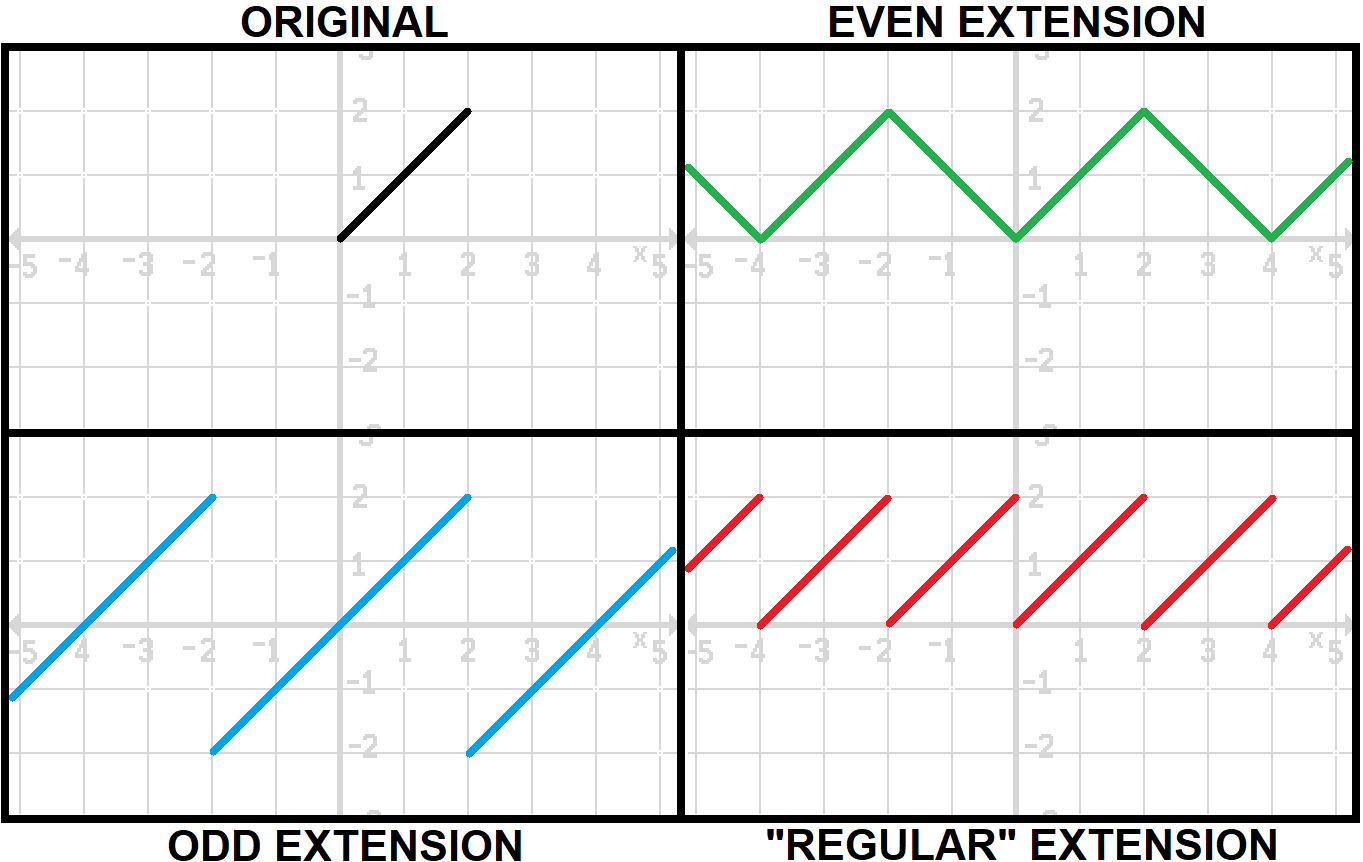
\includegraphics[width=.9\linewidth]{./images/function-extensions.png}
\end{center}

\subsection{Complex Fourier series}
\label{sec:org102cd7f}
Let \(f(x)\) be a periodic function with period \(2L, L \in \mathbb{R}^{+}\). The complex Fourier series of \(f(x)\) is given by:
\[c_0 + \sum_{n = - \infty}^{\infty} c_n e^{\frac{i n \pi x}{L}}, \quad i = \sqrt{-1}\]

Where:
\[c_0 = \frac{1}{2L} \int_{\alpha}^{\alpha + 2L} f(x) \, dx\]
\[c_n = \frac{1}{2L} \int_{\alpha}^{\alpha + 2L} f(x) e^{- \frac{i n \pi x}{L}} \, dx \text{ for } n = 0, \pm 1, \pm 2, \pm 3, \ldots \]

\subsection{Laplace transform of a function (\(\mathcal{L}\))}
\label{sec:org600fed5}
Let \(f(t)\) be a well-defined function for \(t \ge 0\). The Laplace transform is given by:
\[\mathcal{L} \{ f(t) \} = \int_{t = 0}^{t \rightarrow \infty} f(t) e^{-st} \, dt\]

Where:
\begin{itemize}
\item \(s\) is the Laplace transform parameter
\end{itemize}

\subsection{Inverse Laplace transform (\(\mathcal{L}^{-1}\))}
\label{sec:orgf7c39aa}
The inverse Laplace transform is given by:
\[\mathcal{L}^{-1} \{ F(s) \} = f(t)\]

\subsection{Heaviside unit step function (\(u(t - a)\))}
\label{sec:orgfc51df2}
\label{org347bf95}
\begin{displaymath}
u(t - a) = \begin{cases}
0 & \text{for } t \le a \\
1 & \text{for } t > a
\end{cases}
\end{displaymath}

\subsubsection{Difference of two Heaviside unit step functions}
\label{sec:orge7ffa0b}
\begin{displaymath}
u(t - \alpha) - u(t - \beta) = \left. \begin{cases}
1 & \text{for } \alpha < t < \beta \\
0 & \text{for } t < \alpha \text{ or } t > \beta
\end{cases} \right\} \text{ for } 0 \le \alpha < \beta
\end{displaymath}

 \newpage

\section{Other coordinate systems}
\label{sec:org4cd9689}

\subsection{Polar coordinates}
\label{sec:org598e41e}
\begin{center}
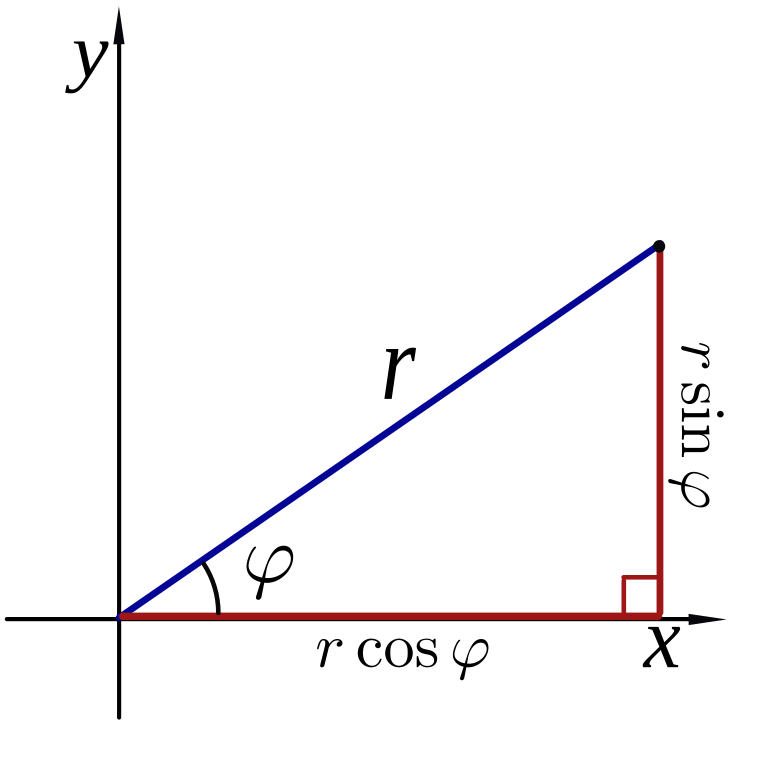
\includegraphics[width=.9\linewidth]{./images/polar-coordinates.png}
\end{center}
\[x = r \cos \varphi\]
\[y = r \sin \varphi\]
\[\text{Infinitesimal area element, } dA = dx dy = r dr d \varphi\]

\subsection{Cylindrical coordinates}
\label{sec:org9f0c36a}
\begin{center}
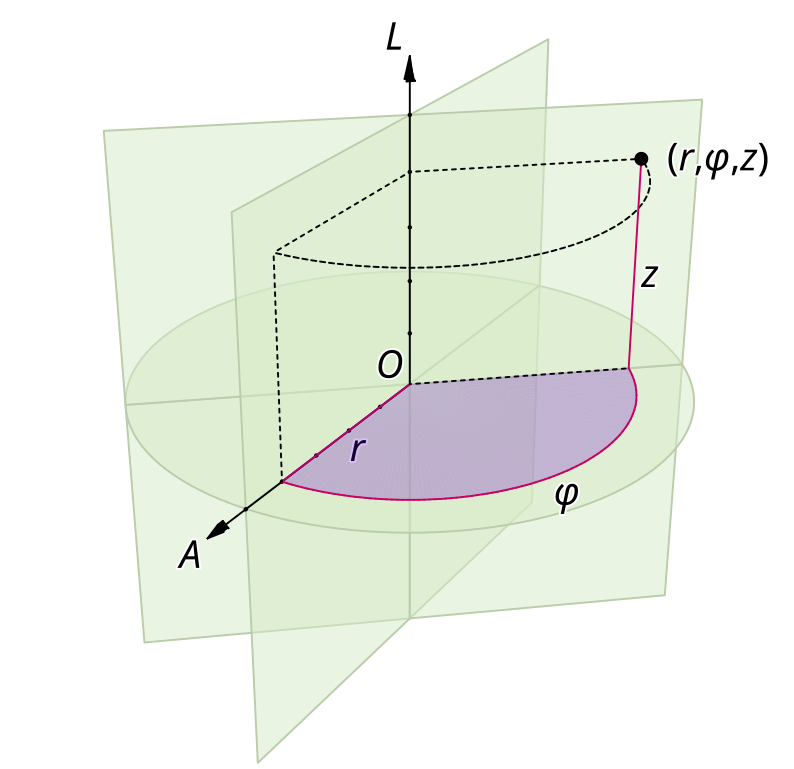
\includegraphics[width=.9\linewidth]{./images/cylindrical-coordinates.png}
\end{center}
\[x = r \cos \varphi\]
\[y = r \sin \varphi\]
\[z = z\]
\[\text{Infinitesimal volume element, } dV = dx dy dz = r dr d \varphi dz\]

\subsection{Spherical coordinates}
\label{sec:org0ab190d}
\begin{center}
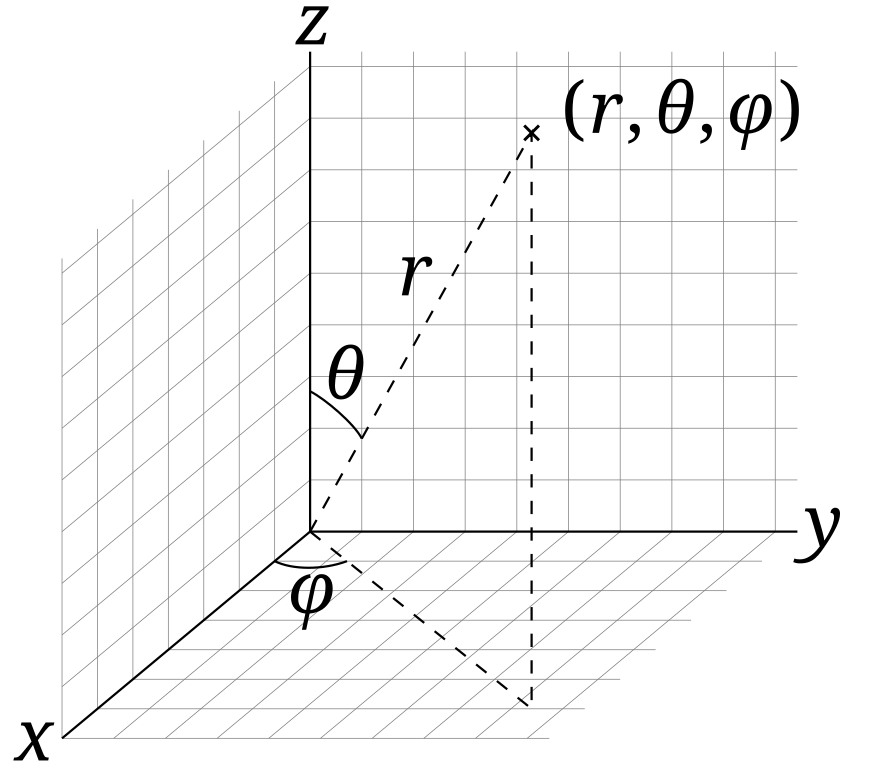
\includegraphics[width=.9\linewidth]{./images/spherical-coordinates.png}
\end{center}
\[x = r \cos \varphi \sin \theta\]
\[y = r \sin \varphi \sin \theta\]
\[z = r \cos \theta\]
\[\text{Infinitesimal volume element, } dV = dx dy dz = r^2 dr d \varphi d \theta\]

 \newpage

\section{Figuring out the integration limits for multiple integrals in Cartesian coordinates}
\label{sec:org4637198}
\begin{enumerate}
\item Choose a variable to integrate with respect to first. For a function \(f(x, y)\), it can be either \(x\) or \(y\).
\item Keep the other variable constant. If we choose \(x\), we keep \(y\) constant, and if we choose \(y\), we keep \(x\) constant.
\item Draw a lot of lines to cover the region \(R\) in the axis of the variable that is kept constant. If \(y\) is kept constant, we draw a lot of \textbf{horizontal lines}. If \(x\) is kept constant, we draw a lot of \textbf{vertical lines}.
\end{enumerate}

\subsection{Example of the 3rd step}
\label{sec:org7bf772f}
The example below is \(\iint_R (3x^2 + y) \, dA\), where \(R\) is the region bounded by the curve \(y = x^2\), the line \(x = 2\) and the positive \(x\)-axis.

\subsubsection{Keeping \(y\) constant}
\label{sec:org1721306}
\begin{center}
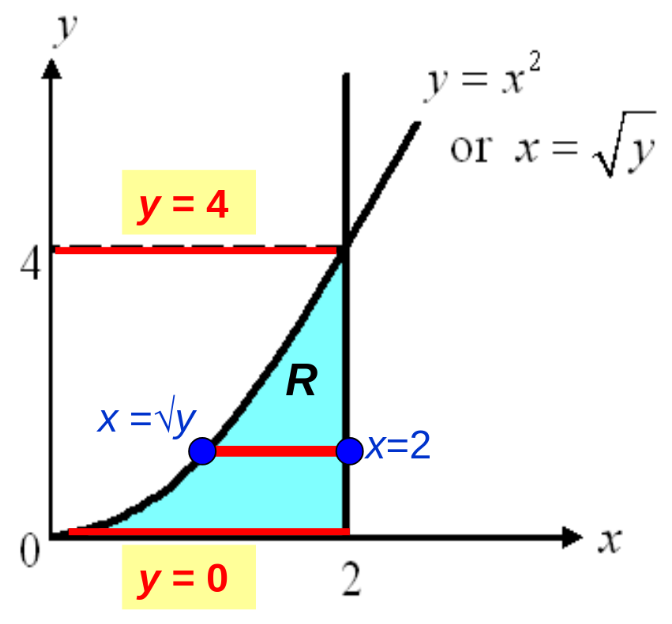
\includegraphics[height=20em]{./images/double-integral-hold-y-constant.png}
\end{center}
\begin{itemize}
\item We can see that the first \textbf{horizontal line} is \(y = 0\) and the last \textbf{horizontal line} is \(y = 4\).
\item Each \textbf{horizontal line} starts on the curve \(x = \sqrt{y}\) and ends on the line \(x = 2\).
\end{itemize}

\subsubsection{Keeping \(x\) constant}
\label{sec:org60cdd8d}
\begin{center}
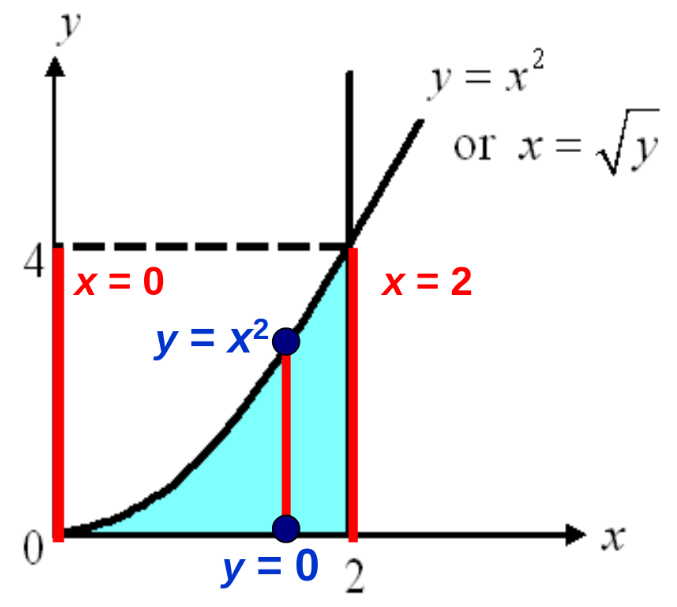
\includegraphics[height=20em]{./images/double-integral-hold-x-constant.png}
\end{center}
\begin{itemize}
\item We can see that the first \textbf{vertical line} is \(x = 0\) and the last \textbf{vertical line} is \(x = 2\).
\item Each \textbf{vertical line} starts on the line \(y = 0\) and ends on the curve \(y = x^2\).
\end{itemize}

\section{Figuring out the integration limits for multiple integrals in polar coordinates}
\label{sec:org85aa587}
\begin{enumerate}
\item Choose a variable to integrate with respect to first. For a function \(f(r, \theta)\), it can be either \(r\) or \(\theta\).
\item Keep the other variable constant. If we choose \(r\), we keep \(\theta\) constant, and if we choose \(\theta\), we keep \(r\) constant.
\item Draw a lot of lines to cover the region \(R\) in the axis of the variable that is kept constant. If \(\theta\) is kept constant, we draw a lot of \textbf{radial lines}, which are lines that come outwards from the centre of the circle. If \(r\) is kept constant, we draw a lot of \textbf{concentric circles} whose radii slowly increases.
\end{enumerate}

\subsection{Example of the 3rd step}
\label{sec:orgffd510f}
The example below is \(\iint_R x^2 + y^2 \, dA\), where \(R\) is the region bounded by the equation \(x^2 + y^2 \le 1\), the line \(x = 0\) and line \(y = 0\).  \\

In polar form, the equation would be:
\[\iint_R (r \cos^2 \theta + r \sin^2 \theta) \, r dr d \theta\]

\subsubsection{Keeping \(\theta\) constant}
\label{sec:orgb1fb62a}
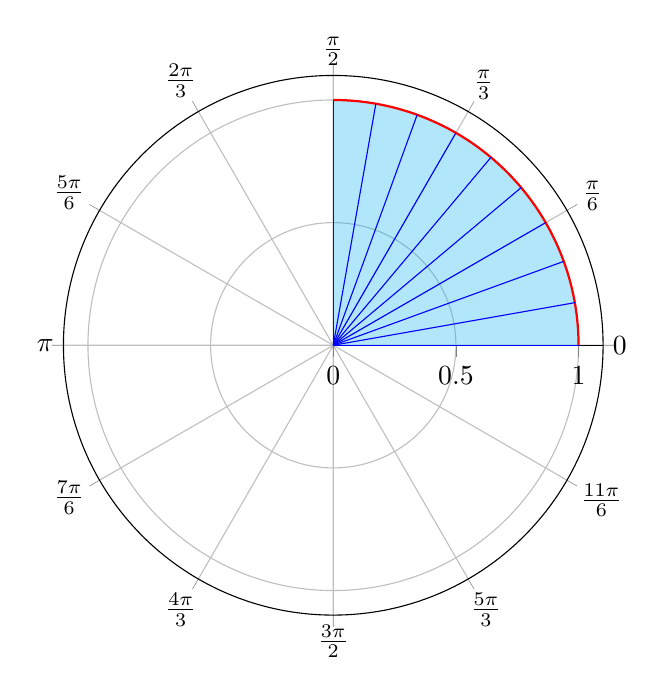
\begin{tikzpicture}
\begin{polaraxis}[
xticklabels={
,0,$\frac\pi6$,$\frac\pi3$,$\frac\pi2$,$\frac{2\pi}3$,$\frac{5\pi}6$,
$\pi$,$\frac{7\pi}6$,$\frac{4\pi}3$,$\frac{3\pi}2$,$\frac{5\pi}3$,$\frac{11\pi}6$
},
ytick align = outside,
yticklabel style = {
anchor = north,
yshift = -2 * \pgfkeysvalueof{/pgfplots/major tick length}
}
]

% The plot of the graph
\addplot [
thick,
name path = f,
domain = 0:90,
samples = 100,
color = red
] {1};

% Invisible axis to fill between
\path[
thick,
name path = axis,
] (axis cs: 0,0) -- (axis cs: 0,1);

% Fill the region
\addplot[
fill = cyan,
fill opacity = 0.3
]
fill between[
of=f and axis
];

% Radial lines
\draw[color = blue] (axis cs: 0,0) -- (axis cs: 0,1);
\draw[color = blue] (axis cs: 0,0) -- (axis cs: 10,1);
\draw[color = blue] (axis cs: 0,0) -- (axis cs: 20,1);
\draw[color = blue] (axis cs: 0,0) -- (axis cs: 30,1);
\draw[color = blue] (axis cs: 0,0) -- (axis cs: 40,1);
\draw[color = blue] (axis cs: 0,0) -- (axis cs: 50,1);
\draw[color = blue] (axis cs: 0,0) -- (axis cs: 60,1);
\draw[color = blue] (axis cs: 0,0) -- (axis cs: 70,1);
\draw[color = blue] (axis cs: 0,0) -- (axis cs: 80,1);
\draw[color = blue] (axis cs: 0,0) -- (axis cs: 90,1);

\end{polaraxis}
\end{tikzpicture}

\begin{itemize}
\item We can see that the first \textbf{radial line} is \(\theta = 0\) and the last \textbf{horizontal line} is \(\theta = \frac{\pi}{2}\).
\item Each \textbf{radial line} starts at the point \(r = 0\) and ends on the circular arc \(r = 1\).
\end{itemize}

\subsubsection{Keeping \(r\) constant}
\label{sec:org328bbf5}
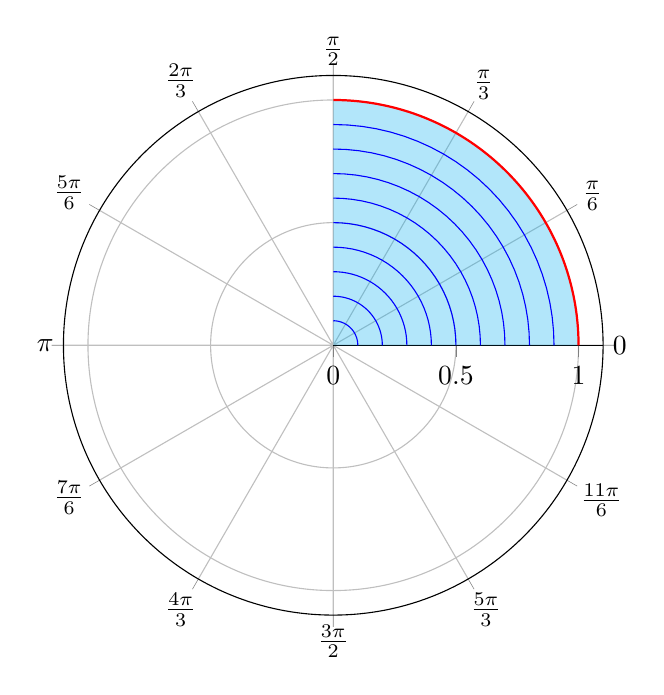
\begin{tikzpicture}
\begin{polaraxis}[
xticklabels={
,0,$\frac\pi6$,$\frac\pi3$,$\frac\pi2$,$\frac{2\pi}3$,$\frac{5\pi}6$,
$\pi$,$\frac{7\pi}6$,$\frac{4\pi}3$,$\frac{3\pi}2$,$\frac{5\pi}3$,$\frac{11\pi}6$
},
ytick align = outside,
yticklabel style = {
anchor = north,
yshift = -2 * \pgfkeysvalueof{/pgfplots/major tick length}
}
]

% The plot of the graph
\addplot [
thick,
name path = f,
domain = 0:90,
samples = 100,
color = red
] {1};

% Invisible axis to fill between
\path[
thick,
name path = axis,
] (axis cs: 0,0) -- (axis cs: 0,1);

% Fill the region
\addplot[
fill = cyan,
fill opacity = 0.3
]
fill between[
of=f and axis
];

% Circles
\addplot[color = blue, domain = 0:90] {0.1};
\addplot[color = blue, domain = 0:90] {0.2};
\addplot[color = blue, domain = 0:90] {0.3};
\addplot[color = blue, domain = 0:90] {0.4};
\addplot[color = blue, domain = 0:90] {0.5};
\addplot[color = blue, domain = 0:90] {0.6};
\addplot[color = blue, domain = 0:90] {0.7};
\addplot[color = blue, domain = 0:90] {0.8};
\addplot[color = blue, domain = 0:90] {0.9};

\end{polaraxis}
\end{tikzpicture}

\begin{itemize}
\item We can see that the first \textbf{concentric circle} is \(r = 0\) and the last \textbf{concentric circle} is \(r = 1\).
\item Each \textbf{concentric circle} starts at the line \(\theta = 0\) and ends on the line \(\theta = \frac{\pi}{2}\).
\end{itemize}

 \newpage

\section{Mathematical formulas}
\label{sec:org9cee5ad}

\subsection{Trigonometric identities}
\label{sec:org8a6621e}

\subsubsection{Basic and Pythagorean identities}
\label{sec:orgb3c01cc}
\[\csc x = \frac{1}{\sin x}\]
\[\sec x = \frac{1}{\cos x}\]
\[\cot x = \frac{1}{\tan x}\]
\[\sin (-x) = - \sin x\]
\[\cos (-x) = \cos x\]
\[\tan (-x) = - \tan x\]
\[\tan x = \frac{\sin x}{\cos x}\]
\[\cot x = \frac{\cos x}{\sin x}\]
\[\sin^2 x + \cos^2 x = 1\]
\[\tan^2 x + 1 = \sec x\]
\[1 + \cot^2 x = \csc^2 x\]

\subsubsection{Angle sum and different identities}
\label{sec:org7be8952}
\[\sin(A \pm B) = \sin A \cos B \pm \cos A \sin B\]
\[\sin(A \pm B) = \cos A \cos B \mp \sin A \sin B\]
\[\tan(A \pm B) = \frac{\tan A \pm \tan B}{1 \mp \tan A \tan B}\]

\subsubsection{Double angle identities}
\label{sec:org90d27f2}
\[\sin 2A = 2 \sin A \cos A\]
\[\cos 2A = \cos^2 A - \sin^2 A = 2 \cos^2 A - 1 = 1 - 2 \sin^2 A\]
\[\tan 2A = \frac{2 \tan A}{1 - \tan^2 A}\]

\subsubsection{Half angle identities}
\label{sec:orgd6c2bd1}
\[\sin \left(\frac{x}{2} \right) = \pm \sqrt{\frac{1 - \cos x}{2}}\]
\[\cos \left(\frac{x}{2} \right) = \pm \sqrt{\frac{1 + \cos x}{2}}\]
\[\tan \left(\frac{x}{2} \right) = \pm \sqrt{\frac{1 - \cos x}{1 + \cos x}} = \frac{1 - \cos x}{\sin x} = \frac{\sin x}{1 + \cos x}\]

\[\sin^2 x = \frac{1}{2} \left[1 - \cos 2x \right]\]
\[\cos^2 x = \frac{1}{2} \left[1 + \cos 2x \right]\]
\[\tan^2 x = \frac{1 - \cos 2x}{1 + \cos 2x}\]

\subsubsection{Sum identities}
\label{sec:orge6fbe70}
\[\sin P + \sin Q = 2 \sin \frac{1}{2}(P + Q) \cos \frac{1}{2}(P - Q)\]
\[\sin P - \sin Q = 2 \cos \frac{1}{2}(P + Q) \sin \frac{1}{2}(P - Q)\]
\[\cos P + \cos Q = 2 \cos \frac{1}{2}(P + Q) \cos \frac{1}{2}(P - Q)\]
\[\cos P - \cos Q = - 2 \sin \frac{1}{2}(P + Q) \sin \frac{1}{2}(P - Q)\]

\subsection{Standard derivatives}
\label{sec:orgc328dd0}
\[\frac{d}{dx} \left(\arcsin x \right) = \frac{1}{\sqrt{1 - x^2}}\]
\[\frac{d}{dx} \left(\arccos x \right) = - \frac{1}{\sqrt{1 - x^2}}\]
\[\frac{d}{dx} \left(\arctan x \right) = \frac{1}{1 + x^2}\]
\[\frac{d}{dx} \left(\csc x \right) = - \csc x \cot x\]
\[\frac{d}{dx} \left(\sec x \right) = \sec x \tan x\]

\subsection{Standard integrals}
\label{sec:org02edf22}
\[\int \frac{1}{x^2 + a^2} \, dx = \frac{1}{a} \arctan \left(\frac{x}{a} \right)\]
\[\int \frac{1}{\sqrt{a^2 - x^2}} \, dx = \arcsin \left(\frac{x}{a} \right)\]
\[\int \frac{1}{x^2 - a^2} \, dx = \frac{1}{2a} \ln \left|\frac{x - a}{x + a} \right|\]
\[\int \frac{1}{a^2 - x^2} \, dx = \frac{1}{2a} \ln \left|\frac{a + x}{a - x} \right|\]
\[\int \frac{1}{\sqrt{x^2 - a^2}} \, dx = \ln \left|\sqrt{x^2 - a^2} + x \right|\]
\[\int \tan x \, dx = \ln |\sec x|\]
\[\int \cot x \, dx = \ln |\sin x|\]
\[\int \csc x \, dx = - \ln |\csc x + \cot x|\]
\[\int \sec x \, dx = - \ln |\sec x + \tan x|\]
\[\int x \cos (px) \, dx = \frac{1}{p^2} (\cos (px) + px \sin (px))\]
\[\int x \sin (px) \, dx = \frac{1}{p^2} (\sin (px) - px \cos (px))\]

 \newpage

\section{Laplace transforms}
\label{sec:orgc8a4293}

\subsection{Elementary functions}
\label{sec:orgb47a255}
\[\mathcal{L} \{ e^{at} \} = \frac{1}{s - a} \text{ for } s > a\]
\begin{center}
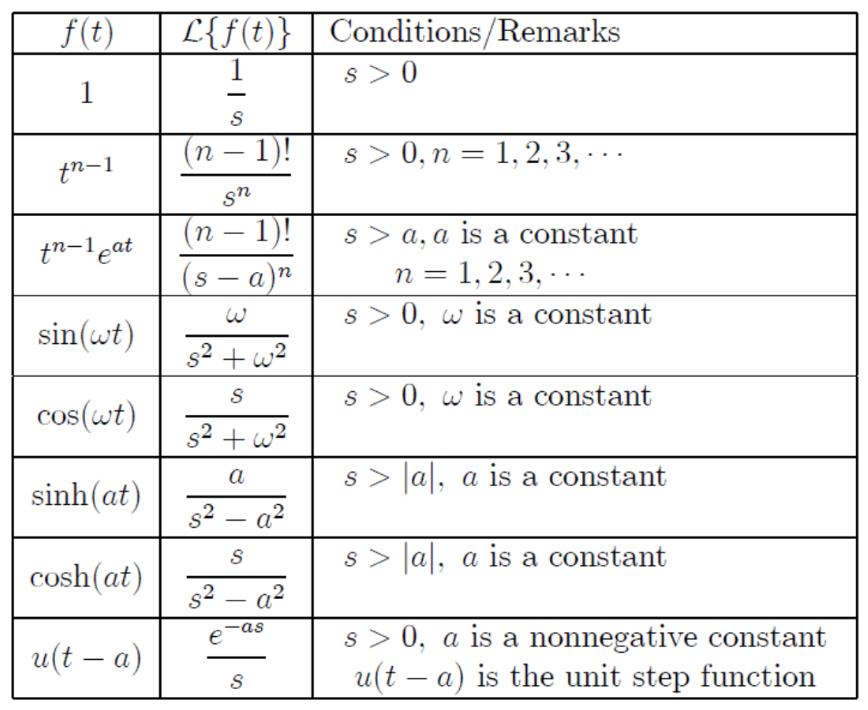
\includegraphics[width=.9\linewidth]{./images/laplace-transform-of-elementary-functions.png}
\end{center}

 \newpage

\subsection{Properties}
\label{sec:org8825b0b}
\begin{itemize}
\item Suppose \(\mathcal{L} \{ f(t) \}\) and \(\mathcal{L} \{ g(t) \}\) exists for \(s > c_f\) and \(s > c_g\) respectively, then:
\[\mathcal{L} \{ \alpha f(t) + \beta g(t) \} = \alpha \mathcal{L} \{ f(t) \} + \beta \mathcal{L} \{ g(t) \} \text{ for } s > \max (c_f, c_g), \quad \alpha, \beta \in \mathbb{R}\]

\item Suppose \(\mathcal{L} \{ f(t) \} = F(s)\) for \(s > c_f\), then:
\[\mathcal{L} \{ e^{at} f(t) \} = F(s - a) \text{ for } s > a + c_f, \quad a \in \mathbb{R}\]

\item Suppose \(\mathcal{L} \{ f(t) \} = F(s)\) for \(s > c_f\), then:
\[\mathcal{L} \{ t^n f(t) \} = (-1)^n \frac{d^n F}{ds^n} \text{ for } s > c_f, \quad n = 1, 2, 3, \ldots\]

\item Suppose \(\mathcal{L} \{ f(t) \}\) exists for \(s > c_f\), then for \(s > c_f\):
\[\mathcal{L} \left\{ \frac{df}{dt} \right\} = s \mathcal{L} \{ f(t) \} - f(0)\]
\[\mathcal{L} \left\{ \frac{d^2 f}{dt^2} \right\} = s^2 \mathcal{L} \{ f(t) \} - sf(0) - f'(0)\]
\[\mathcal{L} \left\{ \frac{d^3 f}{dt^3} \right\} = s^3 \mathcal{L} \{ f(t) \} - s^2f(0) - sf'(0) - f''(0)\]

\item Suppose \(\mathcal{L} \{ f(t) \}\) exists for \(s > c_f\), then:
\[\mathcal{L} \{ u(t - a) f(t - a) \} = e^{-as} F(s) \text{ for } s > c_f, \quad a \ge 0\]

Where:
\begin{itemize}
\item \(u\) is the \hyperref[org347bf95]{Heaviside unit step function}
\end{itemize}

\item Suppose \(\mathcal{L} \{ f(t) \}\) exists for \(s > c_f\), then:
\[\mathcal{L} \left\{ \int_{\tau = 0}^{\tau = t} f(\tau) \, d \tau \right\} = \frac{1}{s} F(s) \text{ for } x > \max (0, c_f)\]
\end{itemize}

\subsection{Table of properties}
\label{sec:org55fc46c}
\begin{center}
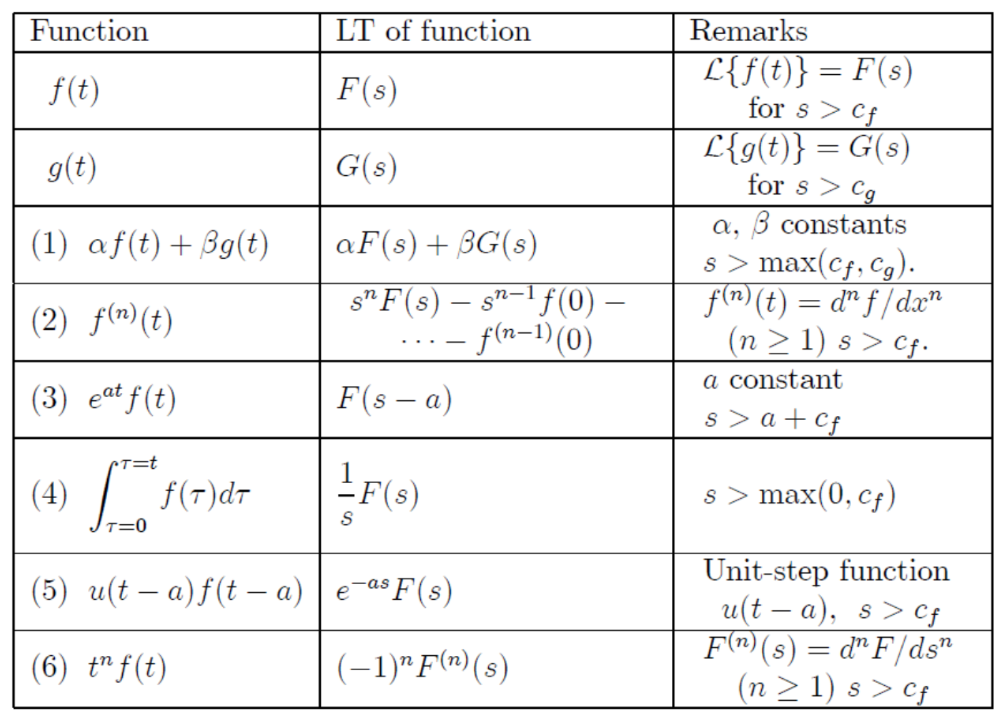
\includegraphics[width=.9\linewidth]{./images/laplace-transform-properties.png}
\end{center}
\end{document}
